\documentclass[a4paper,titlepage,onecolumn,twoside,12pt]{scrreprt}

\usepackage[utf8]{inputenc} %unix-windows-compatible
\usepackage[ngerman,english]{babel} %automatic text in german
\usepackage[
backend=biber,
style=alphabetic,
sorting=ynt
]{biblatex}

\addbibresource{references.bib} %Imports bibliography file

\usepackage{amsmath}
\newcommand{\estimates}{\overset{\scriptscriptstyle\wedge}{=}}

%today command
\newcommand{\leadingzero}[1]{\ifnum #1<10 0\the#1\else\the#1\fi}
\newcommand{\todayGerman}{\leadingzero{\day}.\leadingzero{\month}.\the\year}

%%% LISTINGS
\usepackage{listings}
\usepackage{xcolor}

% acronyms
\usepackage{acronym}

\definecolor{codegreen}{rgb}{0,0.6,0}
\definecolor{codegray}{rgb}{0.5,0.5,0.5}
\definecolor{codepurple}{rgb}{0.58,0,0.82}
\definecolor{backcolour}{HTML}{EEEEEE}
\lstdefinestyle{mylststyle}{
    backgroundcolor=\color{backcolour},   
    commentstyle=\color{codegreen},
    keywordstyle=\color{magenta},
    numberstyle=\tiny\color{codegray},
    stringstyle=\color{codepurple},
    basicstyle=\ttfamily\footnotesize,
    breakatwhitespace=false,         
    breaklines=true,                 
    captionpos=b,                    
    keepspaces=true,                 
    numbers=none,                    
    numbersep=5pt,                  
    showspaces=false,                
    showstringspaces=false,
    showtabs=false,                  
    tabsize=2
}

\colorlet{punct}{red!60!black}
\definecolor{background}{HTML}{EEEEEE}
\definecolor{delim}{RGB}{20,105,176}
\colorlet{numb}{magenta!60!black}

\lstdefinelanguage{json}{
    literate=
     *{0}{{{\color{numb}0}}}{1}
      {1}{{{\color{numb}1}}}{1}
      {2}{{{\color{numb}2}}}{1}
      {3}{{{\color{numb}3}}}{1}
      {4}{{{\color{numb}4}}}{1}
      {5}{{{\color{numb}5}}}{1}
      {6}{{{\color{numb}6}}}{1}
      {7}{{{\color{numb}7}}}{1}
      {8}{{{\color{numb}8}}}{1}
      {9}{{{\color{numb}9}}}{1}
      {:}{{{\color{punct}{:}}}}{1}
      {,}{{{\color{punct}{,}}}}{1}
      {\{}{{{\color{delim}{\{}}}}{1}
      {\}}{{{\color{delim}{\}}}}}{1}
      {[}{{{\color{delim}{[}}}}{1}
      {]}{{{\color{delim}{]}}}}{1},
}


\usepackage{verbatim} %for long comments
\usepackage{latexsym} %for symbol font
\usepackage{color,graphicx} %for inserting color and graphics
\graphicspath{ {./images/}{./figures/} }
\usepackage{tabularx}
\usepackage[T1]{fontenc}
\usepackage{textcomp}
\usepackage{ae}
\usepackage{geometry} %for setting the margins
\setcounter{secnumdepth}{4} %numbering of the subsubsections
\setlength{\parindent}{0pt} %no indentation between paragraphs
\setlength{\parskip}{4pt} %space between paragraphs
\usepackage[margin=10pt,font=small,labelfont=bf,]{caption} [2003/12/20]
\frenchspacing % erzeugt ein wenig mehr Platz hinter einem "." so wie im Dt. ueblich
% define the fancy header:
\usepackage{fancyhdr} 
\fancyhf{} % delete current header and footer
\fancyhead[LO]{\bfseries\rightmark}
\fancyhead[RE]{\bfseries\leftmark}%for twoside-option
\renewcommand{\headrulewidth}{0.5pt}
\renewcommand{\footrulewidth}{0pt}
\addtolength{\headheight}{2.5pt} % space for the rule
\fancypagestyle{plain}{%
	\fancyhead{} % get rid of headers on plain pages
	\renewcommand{\headrulewidth}{0pt} % and the line
}
\pagestyle{fancy}
\cfoot{\thepage}

\definecolor{darkblue}{rgb}{0,0,.4}
\definecolor{darkred}{rgb}{.4,0,0}
\definecolor{darkgreen}{rgb}{0,0.4,0}

\usepackage[pdfpagelabels=true
,backref %references in Literatur-Verz.
, hyperfigures
, bookmarksnumbered
, naturalnames
, plainpages=false
]{hyperref}
\usepackage[hidelinks]{hyperref}
%\hypersetup{breaklinks, colorlinks=false, linkcolor=darkblue, menucolor=darkblue, pagecolor=darkblue, urlcolor=darkblue, citecolor=darkgreen}

\usepackage[figure]{hypcap} % a link jumps and focus on the picture and not on the caption


%start chapter on same page
\usepackage{etoolbox}
\makeatletter
\patchcmd{\scr@startchapter}{\if@openright\cleardoublepage\else\clearpage\fi}{}{}{}
\makeatother


\lstset{style=mylststyle}
\begin{document}
% ---------------------------------------------------------------
    \frontmatter
    \pagenumbering{gobble}% Remove page numbers
    \thispagestyle{empty}
\begin{center}

%\vspace*{1.4cm}
{\LARGE \textbf{Technische Universität Berlin}}

\vspace{0.5cm}

{\large Fakultät IV\\[1mm]}
{\large Institut für Wirtschaftsinformatik und Quantitative Methoden\\[1mm]}
{\large Fachgebiet Agententechnologien in betrieblichen Anwendungen und der Telekommunikation\\[5mm]}

\vspace*{1cm}


\includegraphics[width=4cm]{tu_logo}

\vspace*{1.0cm}

{\LARGE Bachelor Thesis}\\

\vspace{1.0cm}
{\LARGE \textbf{Enabling QoS-­Aware Task Execution}}\\
\vspace*{0.3cm}
{\LARGE \textbf{on Distributed Node­-RED Cluster}}\\
\vspace*{0.3cm}
{\LARGE \textbf{for Fog Computing Environments}}\\
\vspace*{1.0cm}
{\LARGE Daniel Sebastian Lienau}
\\
\vspace*{0.5cm}
Matriculation Number: 378170\\
30.09.2019\\ % 	date of submission
\vspace*{1.0cm}

Supervised by\\
Prof. Dr.-Ing. habil. Dr. h.c. Sahin Albayrak\\
\vspace*{0.5cm}
Assistant Supervisor\\
Cem Akpolat


\end{center}

    \newpage\null\thispagestyle{empty}\newpage
    \chapter*{Eidesstattliche Erklärung}
Hiermit erkläre ich, dass ich die vorliegende Arbeit selbstständig und eigenhändig sowie ohne unerlaubte fremde Hilfe und ausschließlich unter Verwendung der aufgeführten Quellen und Hilfsmittel angefertigt habe.\\

Berlin, den \todayGerman\\
\\

……………………………………………………\\
Unterschrift
    \newpage
\section*{Abstract}
Abstract goes here
 
\section*{Abstrakt}
Abstrakt ...

    \cleardoublepage
    \pagenumbering{arabic}
    \tableofcontents
    
% --------------------------------------------------------------

\mainmatter % comment single chapters for faster compilation
    
    \clearpage
    \chapter{Introduction\label{cha:chapter1}}

The number of interconnected devices on the internet is constantly increasing, thus more and more data is exchanged between different participants.
While the internet initially experienced a broad distribution during the 80s thanks to the world wide web service, where mainly personal computers and enterprise servers were involved in the communication, nowadays the number of offered services and online devices is countless.
Over the last few years, \textit{Internet of Things (IoT)} has become very popular and an end to this trend is not predictable.
Thus, the amount of exchanged data over the internet and between network nodes is constantly increasing as well, leading to higher requirements on the overall network infrastructure to ensure a high connection quality with little delays as well as the avoidance network congestion.\\

A common scenario is devices communicating with each other via a cloud server in a big data center, where the physical distance between devices might be relatively far.
Often though, and this is especially the case for IoT scenarios, a lot of data is produced and consumed locally, on the edge of networks.
While this is not a big deal for services which do not have a high real-time requirement, a service that has a high real-time requirement relies on the network connection quality and low delay times between participating devices.
If this cannot be ensured, the service is unusable.
This becomes even more important in applications where personal safety plays a role, for example, a device at the side of the road communicating with an autonomous car and giving instructions to brake.
If these devices were interconnected via a server in the cloud, the delay time would depend on the current network congestion level, resulting in a varying time in delay, thus not ensuring the \textit{quality of service (QoS)}.
This issue is addressed by fog computing.\\

\textit{Fog computing} provides a distributed infrastructure at the edge of the network, resulting in low-latency access and faster response to application requests \cite{mobility-aware-scheduling}.
In a fog infrastructure, there is a variable number of so called fog nodes, which can provide resources like computation or storage.
Fog nodes are usually small devices with limited resources compared to servers in the cloud.
Furthermore, they are not necessarily of the same kind, thus have a different amount of resources available.
For example, one fog node can have a relatively low computation power compared to another fog node.
The challenge here is to distribute the services among different fog nodes while ensuring the QoS requirements are met.
While some services cannot be executed at all on certain nodes due to the lack of resources, other services are competing for resources on other fog nodes.
One solution here is to \textit{decompose} services into smaller \textit{tasks}, so that these tasks can run on different fog nodes.
However, these tasks need to be recomposed thereafter to provide the service as a whole.
This part is called \textit{service composition} and is illustrated in figure \ref{fig:service-composition}.\\

\begin{figure}
    \centering
    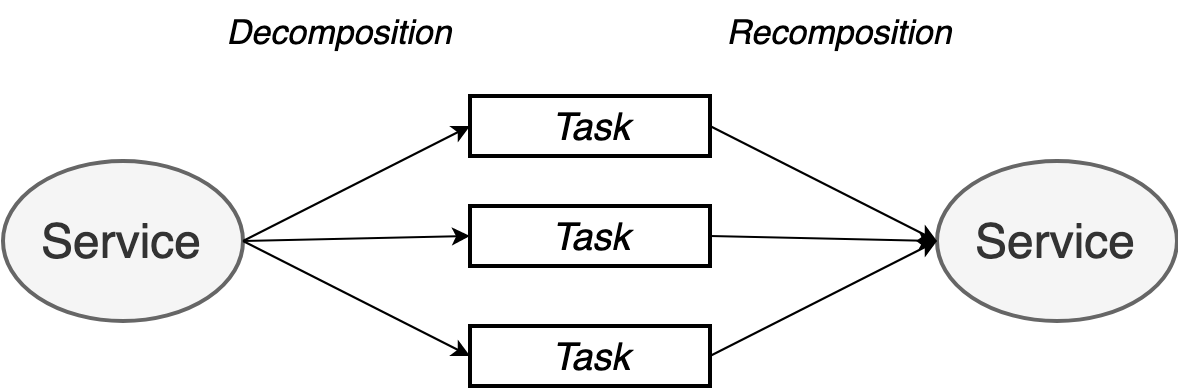
\includegraphics[width=12cm]{service-composition}
    \caption{Service composition}
    \label{fig:service-composition}
\end{figure}

The challenge here is though, that the conditions inside of the fog infrastructure can change at any time.
First of all, the demand for the offered services can increase or decrease at any point in time.
Second, fog nodes can join or leave the network at any point in time.
Simply put, tasks have to be distributed \textit{dynamically}.
To ensure that every service meets the QoS requirements, every node has to be constantly monitored.
If the demand for services increases, the average load on the fog nodes will be high.
To still provide an acceptable service quality for each service, tasks of services which have lower QoS requirements have to be moved to another fog device.
A task could always be executed in the cloud, but this would lead to longer delay times.

    \chapter{Related Work\label{cha:relwork}}
In this section relevant topics for this work are discussed based on related work.

\section{Fog infrastructure}
Fog is an architecture that distributes computation, communication, control and storage closer to the end users along the cloud-to-things continuum \cite{fog-research-opportunities}. Although cloud computing has established itself over the last few years, it cannot be used for certain use-cases, especially time-critical and bandwidth-intensive ones. Because of the closer physical distance to a fog node, fog computing can reach a much lower end-to-end latency than cloud computing \cite{mobility-aware-scheduling}\cite{novel-load-balancing}. This plays a vital role in applications such as vehicle-to-vehicle communication \cite{novel-load-balancing}.\\

A network of fog nodes is a distributed heterogeneous network. Unlike in cloud computing, where hardware capabilities are virtually unlimited \cite{fogtorch}, resources on a fog device are usually constrained. They cannot execute every task because their computation power is limited. Furthermore, the available resources vary from node to node, making the whole network \textit{heterogeneous}. Instead of executing a task on a central computer, it is \textit{distributed} between several nodes in the network.
Firstly, one must determine which fog node can execute which part of the task in terms of resource-constraints.
In the end, all partial results are combined into the final result.\\

Figure \ref{fig:foginfrastructure} shows a typical fog environment.

\begin{figure}
    \centering
    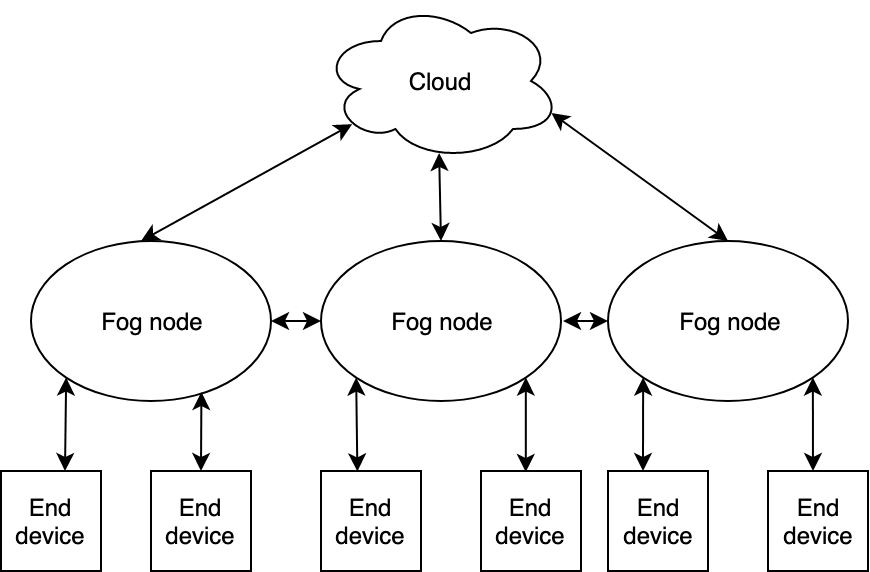
\includegraphics[width=12cm]{fog-computing-infrastructure}
    \caption{Fog infrastructure}
    \label{fig:foginfrastructure}
\end{figure}

\section{Flow-based Programming}
Flow-based programming (FBP) allows the developer to structurally define the informational flow within a system.
As it is not important \textit{where} a specific task is physically executed, FBP focuses on the \textit{path} the data takes from one process to another.
Any number of further processes can be involved in between, while every process manipulates or just reads the data to trigger further actions. Each process has a specific in- and output.
For the developer, all execution units are \textit{black box processes}, which can consume and create data.
The processes can be executed and recomposed in any order, as long as the output and input formats match each other.
It is also possible to split the data flow at a particular point and combine it back together at a later point, making parallel computation possible.\\

Data between processes is transferred in \textit{Information Packets (IPs)}.
IPs belong to a single process or are in a transfer state, where they are owned by no process.
As soon as a process receives an IP, it can start processing it without the need to communicate with other processes, because the IP contains all necessary information the process needs to fulfill the task.
This makes FBP highly attractive for Fog computing environments, where each fog node can be used to execute one or more process types, depending on the process requirements like computation power, bandwidth or latency.

\section{QoS-aware resource allocation and scheduling}
In this section, related work on QoS, load-balancing, and resource allocation is discussed. Although Fog is considered to be a cloud close to the ground, load balancing strategies of cloud computing cannot be directly adopted in the fog network because of the heterogeneity of fog \cite{novel-load-balancing}.

\subsection{FogTorch}
In \cite{fogtorch} a model to support QoS-aware deployment of multicomponent IoT applications to a Fog infrastructures is proposed. Furthermore, a Java tool called \texttt{FogTorch} has been prototyped which implements that model. The model allows to define QoS profiles, Fog infrastructures and IoT applications, which are used to determine eligible deployments.\\

A \texttt{QoS profile} defines bandwidth and average latency required for an application, or offered by a communication link. A \texttt{fog infrastructure} includes IoT devices, Fog nodes, Cloud data centers, and communication links, while each link is associated to its QoS profile. Cloud computing is modeled according to the hypothesis that it can offer a virtually unlimited amount of hardware capabilities. An IoT \texttt{application} is a set of independently deployable components that are working together and must meet some QoS constraints. For this, software components as well as required interactions among components, including the desired QoS profile, are defined. In the end, an \texttt{eligible deployment} for the IoT application is calculated by an algorithm.\\

An algorithm selects where a component is to be deployed within the Cloud to Things continuum. For this, a preprocessing procedure which reduces the search space for eligible deployments runs before a backtracking procedure and heuristics are used to determine a single eligible deployment. Because the proposed backtracking algorithm follows a heuristic approach to get a solution faster, it shows greedy behavior.\\

\cite{fogtorchpi} presents FogTorch$\pi$, an open source prototype based on ForTorch\cite{fogtorch}.
Compared to FogTorch, FogTorch$\pi$ additionally allows for expressing \textit{processing capabilities} and \textit{average QoS attributes} of a Fog infrastructure, as well as processing and QoS requirements of an application.
It determines deployments of the application over the Fog infrastructure that meet all such requirements \cite{fogtorchpi}.
The QoS of communication links are modeled by using probability distributions repeatedly (based on historical data) to simulate different runtime behaviour.
In the end, it aggregates the results for deployments generated over a large number runs.
The output of FogTorch$\pi$ contains eligible deployments (like FogTorch), but additionally outputs QoS assurance and resource consumption over Fog nodes which allows to compare possible deployments and evaluate the impact of possible changes.

\subsection{iFogSim}

In \cite{ifogsim} a tool called \textit{iFogSim} is designed and implemented. It is used to \textit{simulate} a Fog computing environment by using two different placement strategies (\textit{cloud-only} and \textit{edge-ward}). It was found that the average latency of a control loop is much lower in a \textit{edge-ward} than in a \textit{cloud-only} placement strategy.\\

In this work an algorithm for a \textit{real} fog environment is developed and implemented in section \ref{cha:algorithm}, which is inspired by \textit{iFogSim} and adopts some classes of its class model. For this reason, the relevant classes for this work are briefly summarized in the following.\\

\begin{itemize}
    \item \underline{\texttt{FogDevice}}: Specifies hardware characteristics of a node like CPU power, available RAM, available disk storage, as well as network communication capabilities (uplink and downlink).
    
    \item \underline{\texttt{Sensor}}: Represents an IoT sensor, is connected to a \texttt{FogDevice}, has an \textit{output characteristic}.
    
    \item \underline{\texttt{Tuple}}: Fundamental communication unit. It is characterized by its \textit{type}, \textit{source} and \textit{destination} application module. Processing requirements (in \textit{Million Instructions}) and \textit{length of data} are defined as well. 
    
    \item \underline{\texttt{Application}}: An application consists of several modules, each module processing incoming data.
    \begin{itemize}
        \item \underline{\texttt{AppModule}}: Represents processing elements of an application. An instance of an \textit{AppModule} produces an output tuple for every incoming tuple.
        
        \item \underline{\texttt{AppEdge}}: Models the \textit{data-dependency} between a pair of application modules. It is characterized by the \textit{type} of a tuple, \textit{processing requirements} as well as the \textit{length of data} the tuple carries.
        
        \item \underline{\texttt{AppLoop}}: Specifies \textit{process-control loops}. A loop has a \textit{starting} and \textit{terminating} module (as well as any number of modules in between). Figure \ref{fig:apploop} shows an applications containing two loops: \begin{enumerate}
            \item \texttt{Sensor -> Analyzer -> User Interface}
            \item \texttt{Sensor -> Analyzer -> Actuator}
        \end{enumerate}
        For every loop an \textit{end-to-end latency} can be specified. For instance, the second loop might be time critical since an actuator changes the environment based on the sensors value and thus has a lower latency requirement.
    \end{itemize}
\end{itemize}

\begin{figure}
    \centering
    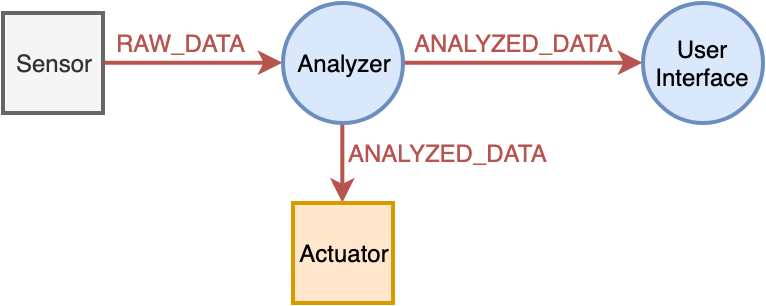
\includegraphics[width=9cm]{algorithm-apploop}
    \caption{Application containing four \texttt{AppModule} and two \texttt{AppLoop} instances}
    \label{fig:apploop}
\end{figure}

\subsection{MPSO-CO}

\cite{novel-load-balancing} proposes the \textit{modified constrained optimization particle swarm optimization} (MPSO-CO) load balancing algorithm, which is \textit{software defined networking} (SDN)-based. Compared to the \textit{constrained optimization particle swarm optimization} (PSO-CO) algorithm, which it is based on, it is able to effectively decrease latency and improve the QoS in a \textit{software defined cloud/fog networking} (SDCFN) architecture. It was developed for applications in the Internet of Vehicles (IoV) which still suffers high processing latency. SDN is used for centralized control and to get the required information before load balancing. The key technology of SDN is decoupling data and control plane. The controller collects real-time information of the network including load, processing speed, and communication latency. Based on that, it can formulate optimal load balancing strategies for the network. It is shown that the MPSO-CO algorithm obtains lower latency compared to PSO-CO, Max-Min load balancing algorithm (LBMM) and greedy load balancing algorithm (Greedy-LB), since LBMM and Greedy-LB do not take the transmission latency into account, and PSO-CO may fall into the local optimum. However, on a low task load (lower than 0.05GB), where transmission latency is not a relevant factor, there is no big difference regarding the latencies of the different algorithms and they all perform pretty much the same.

\section{MAPE-K}
A self-adaptive system consists of the two layers \texttt{managed subsystem} and \texttt{managing subsystem}, whereas the managing subsystem resides on top of the managed subsystem and monitors the managed subsystem as well as the environment. It realizes a feedback loop which adapts to changes, e.g. environmental changes like congestion or failures, or to goal changes \cite{mape-k}.\\

The \textit{Monitor-Analyze-Plan-Execute over a Knowledge base} (MAPE-K) \cite{autonomic-computing} reference control model is the most influential reference control model for autonomic and self-adaptive systems. It is commonly used to realize feedback loops \cite{mape-k}.\\

The component \texttt{Knowledge} (K) is responsible for storing and providing data from/to other components. The component \texttt{Monitor} (M) collects data through probes or sensors from the environment as well as data from the managed subsystem. The collected data is saved in K. The component \texttt{Analyze} (A) analyzes the collected data to check if the system needs to adapt. If this is the case, the component \texttt{Plan} (P) will determine which actions are required to put the system in the desired state. The component \texttt{Execution} (E) then carries out these actions. \cite{mape-k}  
    \chapter{Use Cases\label{cha:use-cases}}

This section describes two different use cases which would benefit from QoS-Aware deployment.

\section{Notify a Device Using Temperature Sensor Data\label{sec:sensordata}}

Sensor networks are used to monitor an (industrial) environment for various measurable parameters. In a \textit{wireless sensor network} (WSN) different types of sensors (e.g. microphones, CO2, pressure, humidity, thermometers) can be used. The measured values are used to decide whether an action should take place or not. Since the sensors themselves usually have few resources for the calculation, this calculation takes place externally. This can be done either centralized or decentralized by distributing the calculation between different nodes.\\

A task execution on a local node rather than on a cloud server makes sense especially for time-critical or data-intensive applications:
\textit{Data-intensive} because the stream of data remains in the local network and does not rely on an internet connection.
Therefore, no bandwidth of the internet connection is occupied.
\textit{Time critical} because the round trip time to a cloud server is usually higher compared to a local server. This work focuses on the time-critical aspect of task distribution and execution.\\

To distribute services between different nodes, a service must first be split into different modules or tasks, which can then be executed on different fog nodes.
In the end, the partial results must be merged to an overall result.
The fog nodes must therefore be able to communicate with each other and forward the final result to another unit, which then takes further action or not based on the result.
The possible actions can be of different priority, e.g. a temperature adjustment might be less important than an emergency stop or emergency braking of a machine.\\

It is very important to use a distributed deployment here because the computational resources of the measurement taking node are limited.
However, the final result of a calculation must be available within a specified time window if time-critical actions have to be executed.
The node itself cannot guarantee to calculate the result in time, so it has to offload the task to another node.\\

\textbf{Use case}:
A factory worker takes products from the conveyor belt.
These could still be hot due to previous processing steps.
A sensor measures the temperature of the products and stops the conveyor belt if necessary to ensure the worker's safety.\\

\textbf{Task}: Notify a device using sensor data
\begin{itemize}
    \item Collect raw data from devices. Devices can be simulated. If a dataset that can be used by these services is found, devices can only forward the data to a specified cloud server.
    \item A cloud service should operate some processes. Based on the data structure provided by those sensors, the cloud service should evaluate different parameters and end up with a result that will be used by another local service/device in the smart factory.\\
\end{itemize}

\textbf{Challenge}: The number of the devices sending data to the cloud service will increase, while the network will be dynamically manipulated through the \texttt{DITG} tool at the same time in order to enforce the Orchestrator to make a decision.
Possible decisions are: Moving the service from a cloud to a fog device, or from one fog to another fog device.

\section{Object Detection}
Object detection is used in most of the fields in daily life.
It is also relevant for a smart factory and factory devices where the information has to be extracted from the recorded picture.
This use case aims at reflecting a simple object detection process that will be operated using an object detection service running in cloud and fog network.
The essential goal is to compare the total delay for the object recognition process in different locations of the network.\\

\textbf{Use case}: Factory prints the products, worker takes the product from the conveyor belt and stores it in one of the container locating in front of the worker.
An IoT-enabled camera tracks the worker object placement to figure out whether the products are placed correctly.
The object detection service should analyze the object and inform the user/robot if there is a mistake while placing the objects.\\

\textbf{Alternative use case}: A factory worker does not know where to place the object, since the objects differ from each other. Therefore, the printed object should be recognized by the object detection service beforehand and then inform the worker in which container the object should be placed.\\

\textbf{Task}: Video processing
\begin{itemize}
    \item Video recording: A local computer sends a video stream to the cloud or to a fog node running an object detection service.
    \item Object detection: The service returns the name of the object in text format as well as the correct container for the object.\\
\end{itemize}

\textbf{Challenge}: The task should first be executed in the cloud. Afterwards, the system should decide if the service requirements are satisfied. Due to varying network conditions which are created by the same tools mentioned in \ref{sec:sensordata}, the system should decide to move the service from the cloud or a fog node to another fog node which can satisfy the service requirements.
    \chapter{Problem Definition \& Challenges\label{cha:problem-definition}}
This part structures the problem. The problem here is mainly resource allocation and its usage. What are the technical and the theoretical challenges?

\section{Load Balancing Among Fog Nodes}
In a Node-RED context, a service can be seen as a Node-RED \textit{flow} and consists of several \textit{tasks} (functions in a flow), whereas each function could be executed on a different node.
The challenge here is to decide which node should execute which function (see figure \ref{fig:distributed-flow}).
The goal is to meet the service's QoS requirements.
For the MWSN use cases it has to be ensured that a result is available within the defined maximum latency timespan, e.g. within 10ms for condition monitoring for safety.\\

\begin{figure}
    \centering
    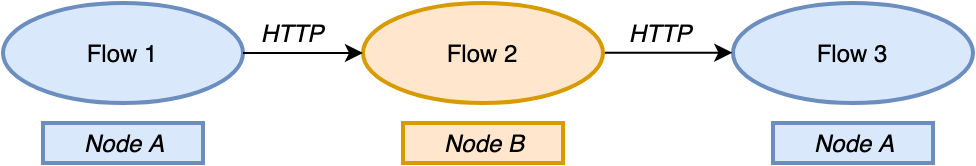
\includegraphics[width=12cm]{architecture-distributed-flow}
    \caption{Distributed flow}
    \label{fig:distributed-flow}
\end{figure}

Fog infrastructure is characterized by different nodes offering various hardware and software resources.
In order to assign tasks to nodes, it must first be checked whether a node is able to execute the task with given QoS requirements.\\

The challenge here is to implement a resource allocation algorithm for the given use cases.


\section{Dynamically Varying Network Conditions}
The network conditions might change at any point in time.
The increased demand for services plays a major role here, but there may also be increased network traffic.
For instance, in the MWSN scenario, the amount of sensors requesting services might increase, which leads to a higher load on the fog nodes hardware until the point of congestion.
To avoid congestion and ensure QoS, tasks of services with a lower priority have to be moved elsewhere to free resources for high priority services.
Apart from that, the network traffic might increase due to other network services which are not part of the fog infrastructure but are using the same link.\\

The challenge here is to adapt to the mentioned changes, for which they must be identified first before the load balancing algorithm is executed to eventually calculate a differentiated, optimized deployment.

\section{Fog Node Failures}
A fog infrastructure is not as reliable as a cloud infrastructure, for instance.
Fog nodes can join or leave the network at any point in time, which leads to a dynamic change in the available resources.
Since fog nodes can be any type of hardware, it is not unlikely that small and relatively cheap devices (e.g. Raspberry Pi) are used.
Thus, it is more likely that they might fail since the hardware components are not of high quality compared to enterprise server hardware.
Furthermore, the environment is neither monitored nor controlled like a cloud server data center, which could lead to node failures (e.g. network connection errors or power supply failures).\\

The challenge here is to adapt to those dynamic changes.
If a node leaves the network, fewer resources are available and therefore another deployment might be the optimum.
Similarly, when a node joins the network, more resources are available, making another deployment ideal.

    \chapter{Design and Implementation of a QoS-Aware Scheduling Algorithm\label{cha:algorithm}}

This section describes the design and implementation of the \textit{QoS Scheduler} which is used in chapter \ref{cha:orchestrator}. UML diagrams can be found in appendix \ref{cha:algorithm-UML-diagrams}.

\section{Algorithm Architecture}

The algorithm takes an \texttt{Infrastructure} and an \texttt{Application} as inputs, and outputs an optimal deployment strategy (\texttt{AppDeployment}).
The optimal deployment strategy differs depending on the type of scheduler.
For example, the goal of a scheduler can be to minimize the total \textit{energy consumption}, the total \textit{network utilization} or the \textit{computing power} used.
Since the focus here is on \textit{QoS}, the deployment that minimizes \textit{total latency} should be the optimal deployment.
Figure \ref{fig:algorithm-architecture} illustrates the architecture of the algorithm.

\begin{figure}[h]
    \centering
    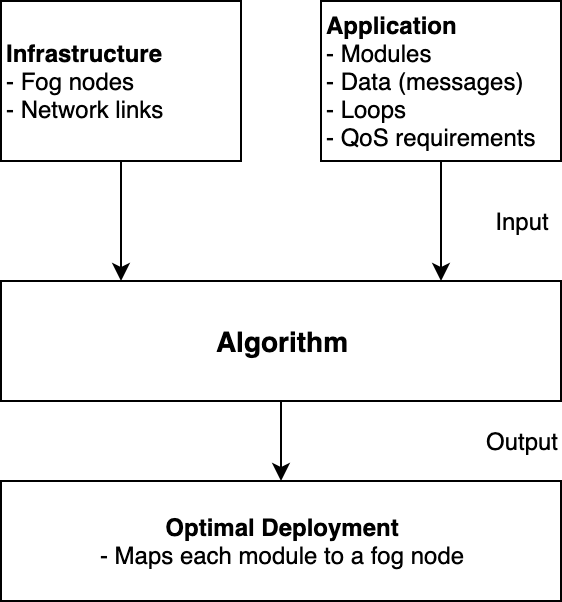
\includegraphics[width=7cm]{algorithm-architecture}
    \caption{QoS scheduling algorithm architecture}
    \label{fig:algorithm-architecture}
\end{figure}


\subsection{Infrastructure\label{sec:algorithm-infrastructure}}

The infrastructure consists of \textit{fog nodes} and \textit{network connections} between those nodes.
Network connections are modeled as uplinks only, because we are sending data forward in the application loop from one module to another, while every module is deployed on one fog node.
Between two nodes (node A and node B), the downlink of node B from node A's point of view is the same as the uplink of node A from node B's point of view.
Therefore, each fog node has a set of uplinks to all other reachable Fog nodes.
A node also has an uplink to itself, since the next module in the loop could be executed on the same node.
This uplink is modeled with \textit{infinite speed} and \textit{zero latency}.
Hence, there are \(n^2\) uplinks in the infrastructure in total ($n \estimates number\ of\ Fog\ nodes$).
Figure \ref{fig:algorithm-infrastructure} shows a fog infrastructure with three nodes and the corresponding nine uplinks.

\begin{figure}[htb]
    \centering
    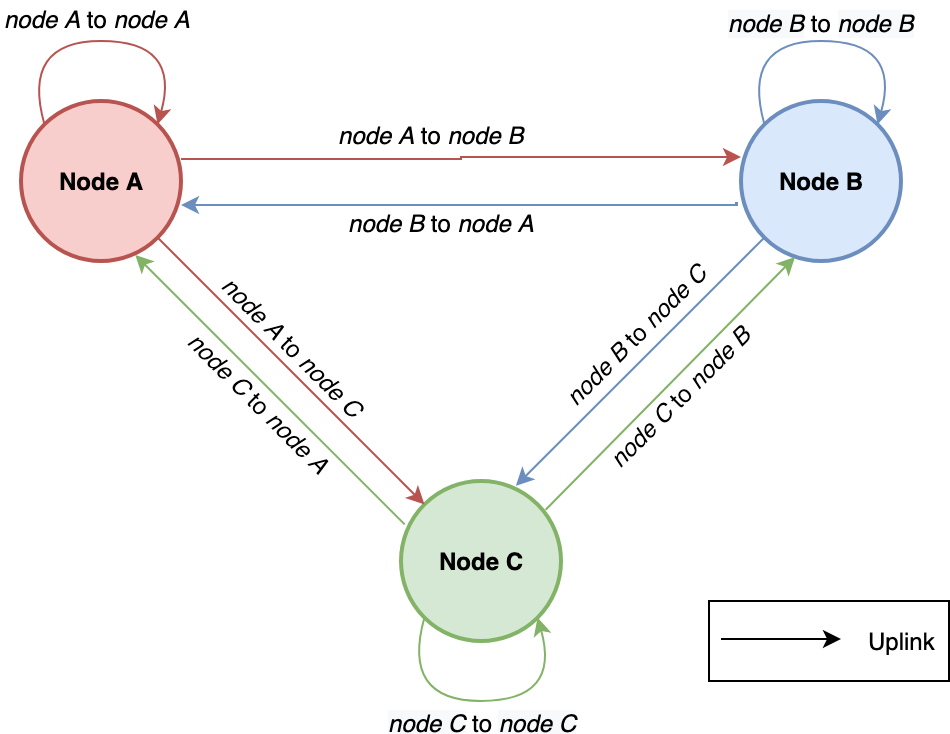
\includegraphics[width=0.75\textwidth]{algorithm-infrastructure}
    \caption{Infrastructure with three nodes and nine uplinks}
    \label{fig:algorithm-infrastructure}
\end{figure}

Next, the relevant classes for the infrastructure are described. The corresponding class diagram is depicted in figure \ref{fig:classdiagram-infrastructure}.

\begin{itemize}
    \item \underline{\texttt{Infrastructure}}: Contains a \texttt{List} of \texttt{FogNode} instances.
    
    \item \underline{\texttt{NetworkUplink}}: Every instance of \texttt{NetworkUplink} has the following \textit{fields}:
    \begin{itemize}
        \item \underline{\texttt{source}}: The source \texttt{FogNode} of the link.
        \item \underline{\texttt{destination}}: The destination \texttt{FogNode} of the link.
        \item \underline{\texttt{latency}}: The RTT of the link.
        \item \underline{\texttt{bitPerSecond}}: The link speed (bandwidth) in bit per second.
    \end{itemize}

    \item \underline{\texttt{FogNode}}: Every instance of \texttt{FogNode} has the following \textit{fields}:
    \begin{itemize}
        \item \underline{\texttt{id}}: The identifier of the device, e.g. its hostname.
        \item \underline{\texttt{ramTotal}}: The total available ram.
        \item \underline{\texttt{storageTotal}}: The total available disk space.
        \item \underline{\texttt{cpuCores}}: The amount of available CPU cores.
        \item \underline{\texttt{cpuMips}}: The power of a CPU measured in MIPS (million instructions per second).
        \item \underline{\texttt{connectedHardware}}: Hardware connected to the node (e.g. camera, temperature sensor)
        \item \underline{\texttt{uplinks}}: Uplinks to other fog nodes (\texttt{NetworkUplink} objects)
    \end{itemize}
    
    Every instance of \texttt{FogNode} has the following \textit{methods}:
    \begin{itemize}
        \item \underline{\texttt{deployModule(AppSoftwareModule module): boolean}}\\ [0.5ex] 
        Tries to deploy an \texttt{AppSoftwareModule} (see section \ref{sec:algorithm-application}) on this node. Checks whether this node can fulfill the modules requirements (RAM, storage, hardware modules). Modules are \textit{not} automatically undeployed. The method can be called multiple times and thus more than one module can be deployed. In this case, sufficient resources must be available to execute \textit{all} modules. The method returns \texttt{false} for the first module that cannot be deployed, otherwise \texttt{true}.
        
        \item \underline{\texttt{getUplinkTo(FogNode destination): NetworkUplink}}\\ [0.5ex] 
        Returns the \texttt{NetworkUplink} from this node to the \texttt{destination} node.
        
        \item \underline{\texttt{calculateProcessingTime(AppSoftwareModule module): double}}\\ [0.5ex] 
        Calculates the execution time of an \texttt{AppSoftwareModule} (see section \ref{sec:algorithm-application}) on this node. Returns the value in milliseconds. The result is calculated using the following formula:
        \[\textrm{execution time [ms]} = \frac{\textrm{\texttt{requiredMi}}}{\textrm{\texttt{cpuMips}}}\ \boldsymbol{\cdot} 1000\]
    \end{itemize}

\end{itemize}


\subsection{Application\label{sec:algorithm-application}}

An application consists of \textit{modules}, \textit{messages} and \textit{loops}. A module can either be a \textit{hardware module} (e.g. a camera or a temperature sensor) or a \textit{software module} (e.g. data processor, object detection engine).

Next, the relevant classes for an application are described. The corresponding class diagram is shown in figure \ref{fig:classdiagram-application}.

\begin{itemize}
    \item \underline{\texttt{AppModule}}: This abstract class is extended by the classes \texttt{AppHardwareModule} and \texttt{AppSoftwareModule}. It contains the following \textit{fields}:
    \begin{itemize}
        \item \underline{\texttt{id}}: The type of this module, e.g. \texttt{CAMERA} (hardware) or \texttt{OBJECT\_DETECTOR} (software).
        \item \underline{\texttt{inputType}}: The modules input type, e.g. \texttt{IMAGE\_RAW} from a camera (can be \texttt{null} for the starting module of a loop).
        \item \underline{\texttt{outputType}}: The modules output type, e.g. \texttt{IMAGE\_PROCESSED} (can be \texttt{null} for the terminating module of a loop).
    \end{itemize}

    \item \underline{\texttt{AppHardwareModule}}: A hardware module extends \texttt{AppModule} and solely consists of the three fields of \texttt{AppModule}. If it has an \texttt{outputType} but no \texttt{inputType}, it is a \textit{sensor} (e.g. temperature sensor, outputs the current temperature). If it has an \texttt{inputType} but no \texttt{outputType}, it is an \textit{actuator} (e.g. air conditioner, takes a target value as input, outputs nothing).
    
    \item \underline{\texttt{AppSoftwareModule}}: A software module extends \texttt{AppModule} and additionally has the following \textit{fields}:
    \begin{itemize}
        \item \underline{\texttt{requiredRam}}: Memory required by the module.
        \item \underline{\texttt{requiredStorage}}: Disk storage required by the module.
        \item \underline{\texttt{requiredHardwareModules}}: Hardware modules that must be connected to the node that executes the software module. For instance, the hardware module \texttt{CAMERA} must be connected to a node which executes the software module \texttt{CAMERA\_CONTROLLER} in order to instruct the camera to take a picture first and output that picture to another module for further processing in the next step.
        \item \underline{\texttt{requiredMi}}: This attribute determines how many CPU instructions (defined in million instructions) are needed approximately for processing a single message. This allows the execution time to be estimated.
    \end{itemize}
    
    \item \underline{\texttt{AppMessage}}: A message has the following \textit{fields}:
    \begin{itemize}
        \item \underline{\texttt{contentType}}: The content of a message, e.g. \texttt{IMAGE\_RAW}, \texttt{IMAGE\_PROCESSED}.
        \item \underline{\texttt{dataPerMessage}}: The data size per message in KByte, e.g. 500 KB for an image.
    \end{itemize}
    A message has the following \textit{methods}:
    \begin{itemize}
        \item \underline{\texttt{transferTime(source: FogNode, destination: FogNode): double}}\\
        Calculates the transfer time of the message based on the \texttt{NetworkUplink} from \texttt{source} node to \texttt{destination} node. Returns the value in milliseconds. The result is calculated using the following formula:
        \[\textrm{transfer time [ms]} = \textrm{latency [ms]} + \frac{\textrm{message size [bit]}}{\textrm{link speed} [\frac{\textrm{bit}}{\textrm{ms}}]}\]
    \end{itemize}
   
   \item \underline{\texttt{AppLoop}}: A loop defines the connection between the different app modules.
   An application can consist of one or more loops, while each loop has a unique \textit{start}, \textit{end}, and \textit{maximum latency}.
   The loop determines how or in which \textit{order} the modules are \textit{connected} to each other.
   The maximum latency attribute defines the maximum allowed duration for one cycle.
   For instance, the loop's last module \texttt{IMAGE\_VIEWER} should view an image not later than \textit{1 second} after the loop's first module \texttt{CAMERA} took the image.
   
   In figure \ref{fig:object-detection-appmodules}, the order is as follows:\\
    \texttt{CAMERA} $\rightarrow$ \texttt{camera-controller} $\rightarrow$ \texttt{object-detector} $\rightarrow$ \texttt{image-viewer}\\[0.5ex]
   A loop has the following \textit{fields}:
   \begin{itemize}
       \item \underline{\texttt{name}}: The name of the loop, e.g. \textit{object-detection}.
       \item \underline{\texttt{maxLatency}}: Time (in milliseconds) in which the result must be available, i.e. the time required to process all modules from the first to the last.
       \item \underline{\texttt{modules}}: A \texttt{LinkedList} containing all modules belonging to this loop. The order of this list determines the execution order of the loop.
   \end{itemize}
   A loop has the following \textit{methods}:
   \begin{itemize}
       \item \underline{\texttt{totalLatency(AppDeployment d): double}}\\
       Calculates the total latency for the loop for a given \texttt{AppDeployment} (see section \ref{sec:algorithm-scheduler}).
       Returns the value in milliseconds. The total latency is the sum of the loop's task executions and its message transfers between modules.
       How these two values are calculated is depicted in figures \ref{fig:algorithm-activitydiagram-latency-processing} and \ref{fig:algorithm-activitydiagram-latency-transfer}.
   \end{itemize}
\end{itemize}

\begin{figure}[htbp]
    \centering
    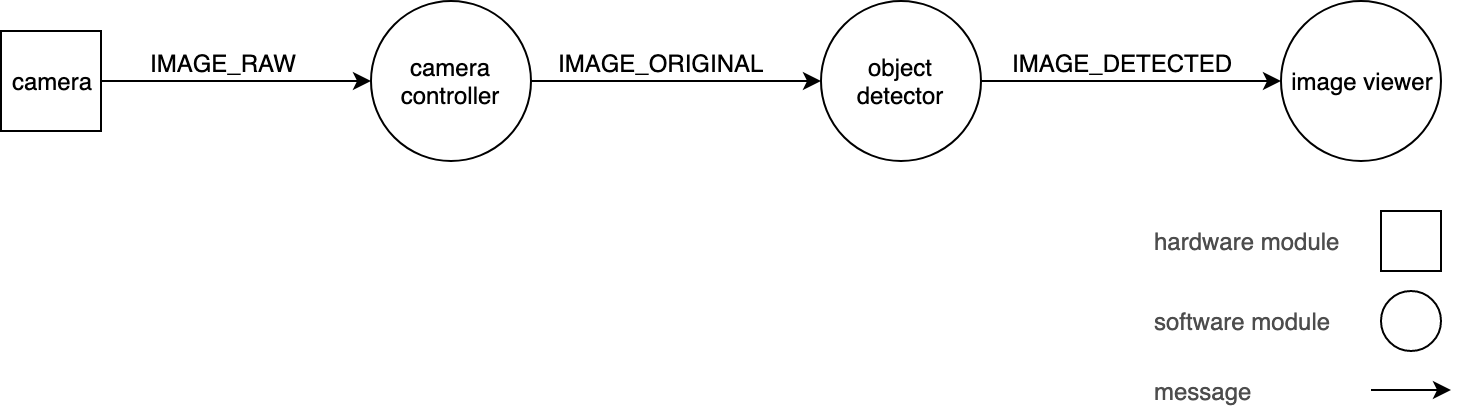
\includegraphics[width=1.0\textwidth]{object-detection-appmodules}
    \caption{Object detection application containing four modules}
    \label{fig:object-detection-appmodules}
\end{figure}

%%%%%%%%%%%%%%%%%%%%%%%%%%%%%%%%%%%%%%
%%%%% SUBSECTION INFRASTRUCTURE %%%%%%
%%%%%%%%%%%%%%%%%%%%%%%%%%%%%%%%%%%%%%


\subsection{Scheduler\label{sec:algorithm-scheduler}}

The architecture includes the interface \texttt{Scheduler}, which has the two methods \texttt{getOptimalDeployment()} and \texttt{getValidDeployments()}. The former method returns the one optimal deployment (\texttt{AppDeployment}), while the latter one returns a list of all possible deployments that meet the requirements. Class relationships are shown in figure \ref{fig:classdiagram-qosscheduler}.

The class \texttt{AppDeployment} is used to represent a deployment for a given \texttt{Application}. The field \texttt{moduleToNodeMap} is used to specify which module (\texttt{AppSoftwareModule}) should be executed on which node (\texttt{FogNode}).

In section \ref{sec:qos-scheduler} the concrete class \texttt{QosScheduler} is described, which implements the \texttt{Scheduler} interface.



\section{QoS Scheduler\label{sec:qos-scheduler}}
The job of the \textit{QoS Scheduler} is to find all deployments which satisfy the latency requirements of all application loops.
It outputs the one deployment with the lowest latency.
This section describes how this task is solved.\\

The \texttt{QosScheduler} takes an \texttt{Application} and an \texttt{Infrastructure} in the constructor.
It tries to find all valid deployments as well as the optimal deployment for the \texttt{Application} over the \texttt{Infrastructure}.

In the first step, the scheduler creates a combination of all possible deployment strategies without checking if the modules could be executed on the assigned nodes (hardware requirements) and if latency requirements are met (app loop requirements).
In a mathematical sense, a permutation with repetition is created in this step.

Table \ref{tab:deployment-combinations} shows all nine possible combinations of an application consisting of \textit{two modules} and an infrastructure consisting of \textit{three fog nodes}.

\begin{table}[htb]
    \centering
    \begin{tabular}{|c||c|c|}
    \hline
        \# & \textbf{module A} & \textbf{module B}\\
         \hline\hline
         1. & node 1 & node 1\\
         \hline
         2. & node 1 & node 2\\
         \hline
         3. & node 1 & node 3\\
         \hline
         4. & node 2 & node 1\\
         \hline
         5. & node 2 & node 2\\
         \hline
         6. & node 2 & node 3\\
         \hline
         7. & node 3 & node 1\\
         \hline
         8. & node 3 & node 2\\
         \hline
         9. & node 3 & node 3\\
         \hline
    \end{tabular}
    \caption{Combination of all possible deployments for an application with two modules and an infrastructure with three nodes}
    \label{tab:deployment-combinations}
\end{table}

Each line represents a \textit{deployment strategy candidate}.
However, it has not yet been checked whether the deployment strategy is valid because the requirements have not been examined yet.
In order to do so, the \textit{QoS Scheduler} goes through several steps to analyze if a deployment strategy fulfills the application requirements.
If the answer to any step is negative, this deployment strategy candidate is not valid and the next one will be analyzed.
How the algorithm creates a set of valid deployments is depicted in \ref{fig:algorithm-activitydiagram-validdeployments}, which is also the implementation of the method \texttt{getValidDeplopyments()}.

\begin{figure}[htb]
    \centering
    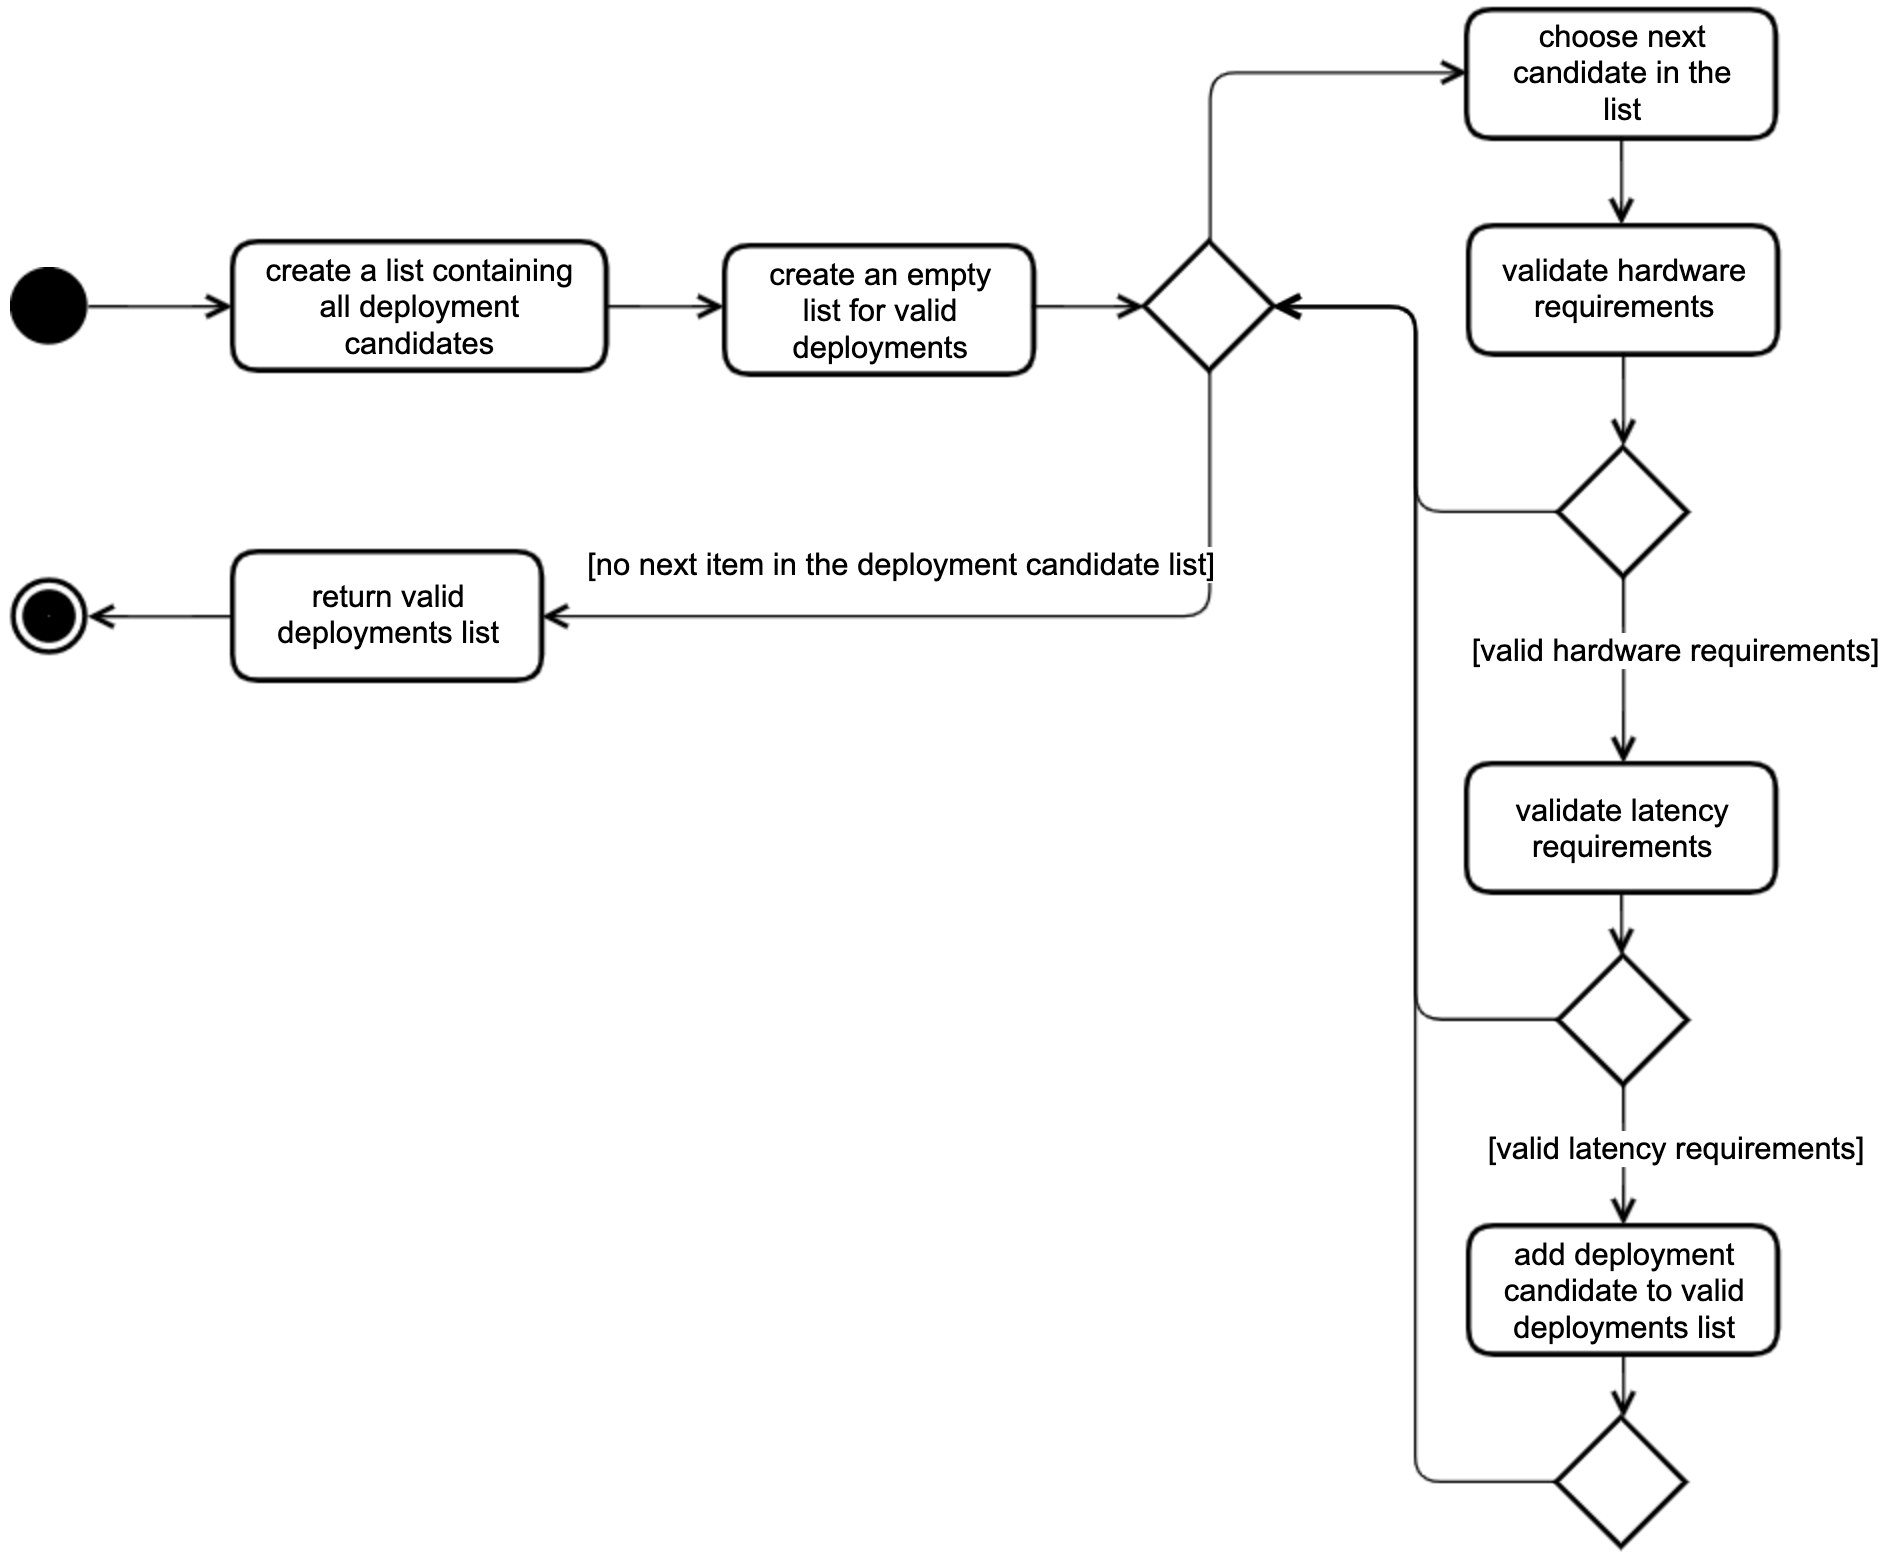
\includegraphics[width=1.0\textwidth]{algorithm-activitydiagram-validdeployments}
    \caption{Activity diagram for finding possible deployments}
    \label{fig:algorithm-activitydiagram-validdeployments}
\end{figure}

The result is a set of deployments which fulfill the application requirements.
The \textit{optimal deployment} is the one with the \textit{lowest total latency} and will be returned by calling the method \texttt{getOptimalDeployment()}.
The corresponding activity diagram is shown in figure \ref{fig:algorithm-activitydiagram-optimaldeployment}.

\begin{figure}[htb]
    \centering
    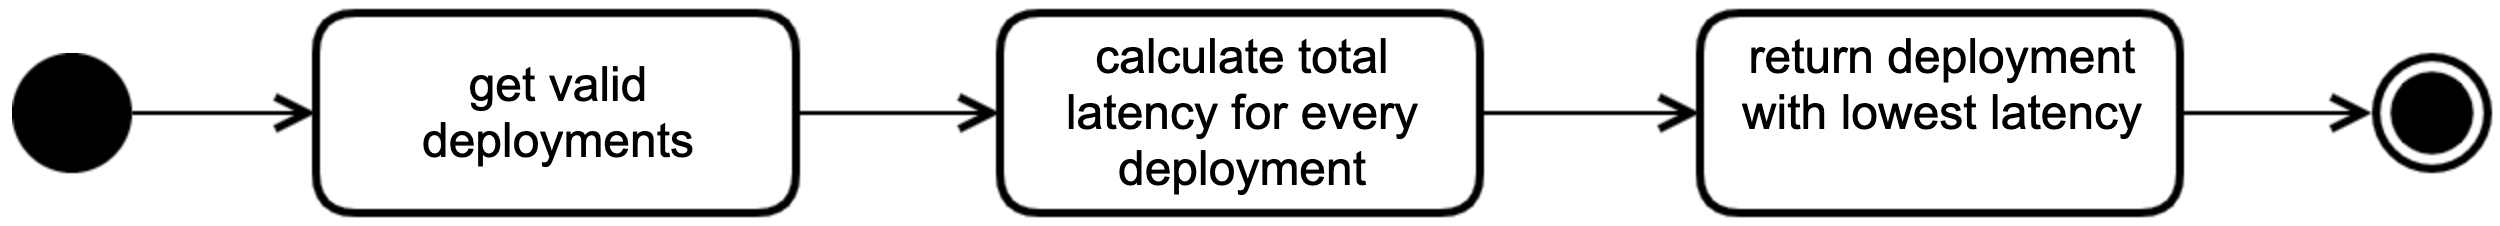
\includegraphics[width=1.0\textwidth]{algorithm-activitydiagram-optimaldeployment}
    \caption{Activity diagram for finding the optimal deployment}
    \label{fig:algorithm-activitydiagram-optimaldeployment}
\end{figure}

How the hardware and latency requirements are validated is shown in figures \ref{fig:algorithm-activitydiagram-hardware} and \ref{fig:algorithm-activitydiagram-latency}.
To validate latency requirements it is necessary to calculate the \textit{total latency} of a loop, which is the sum of the processing times of all modules and all message transfers between the modules of the loop.
The following formula shows the calculation of the total latency with $t_n$ = execution time of module \textit{n}, and $t_m$ = transfer time of message \textit{m}:

\[ \textrm{total latency} = \sum_{n=0}^N t_n + \sum_{m=0}^M t_m\]

The calculations of \textit{total processing time} and \textit{total transfer time} are depicted in figures \ref{fig:algorithm-activitydiagram-latency-processing} and \ref{fig:algorithm-activitydiagram-latency-transfer}.


    \chapter{QoS-Monitor \& -Orchestrator\label{cha:orchestrator}}

The algorithm described in section \ref{cha:algorithm} works so far in a static context. However, the task is to apply the optimal deployment to a Node-RED cluster, where the network conditions can change at any time. While the application characteristics remain unchanged, the infrastructure can change mainly in two ways. First, fog nodes may join or leave the network, and second, network connection quality between nodes can get better or worse. These changes must be detected by the Orchestrator, and if the current deployment strategy no longer meets the application requirements, a new optimal deployment must be found and applied.

The class \texttt{NodeRedOrchestrator} takes care of this job. It monitors the infrastructure and deploys the optimal deployment to it by using the \textit{QoS-Scheduler}. To make use of the \textit{QoS-Scheduler}, an \texttt{Infrastructure} and \texttt{Application} instance must be available. The former one is actively maintained by the Orchestrator (see section \ref{orchestrator-monitoring}), while the latter one is statically created upon start-up of the \texttt{NodeRedOrchestrator}. The class \texttt{FogNode} of the algorithm in section \ref{cha:algorithm} is extended by the class \texttt{NodeRedFogNode} in order to add additional functionality for measuring the nodes hardware and network capabilities before it is added to the infrastructure.

The corresponding class diagram is shown in figure \ref{fig:orchestrator-classdisgram}.

\section{Monitoring the infrastructure\label{orchestrator-monitoring}}

Directly after starting the orchestrator, it is only aware of the applications that should be deployed to the infrastructure. However, the infrastructure is empty at the beginning. Fog nodes send their availability status via a \texttt{heartbeat} message to a \texttt{MQTT} broker at a given interval. The orchestrator listens for those messages and has different handlers for different possibilities:
\begin{enumerate}
    \item The node sending the heartbeat is not registered in the current infrastructure\\
    → Handle new fog node
    \item The node sending the heartbeat is registered\\
    → Update timestamp of last received heartbeat
    \item Orchestrator is expecting but missing a heartbeat from a node\\
    → Check if node is still up and if not, remove it from infrastructure
\end{enumerate}

\subsection*{Handling new fog nodes}

In the case of receiving a heartbeat from a node that the orchestrator does not know yet, the hardware capabilities as well as the network connection of the node must be checked before it can be added to the infrastructure. To achieve this, the node is able to receive several commands via \texttt{MQTT}.

\begin{itemize}
    \item \texttt{sysinfo}: Sends basic information about the nodes hardware (\textit{RAM}, \textit{storage}, \textit{cpu cores}, \textit{connected hardware}).
    \item \texttt{ping}: Measures the \textit{RTT} from this node to another node. Returns the latency in milliseconds. The command line tool \texttt{ping} is used for this purpose.
    \item \texttt{bandwidth}: Measures the network connection from this node to another node. Returns the bandwidth in Mbit/s.
    \item \texttt{benchmark\_cpu}: Runs the tool \texttt{sysbench} which is a lightweight benchmark tool made for linux servers. The result is the \textit{execution time} for a given (but always the same) task. The faster the execution time, the faster the CPU.
\end{itemize}

Figure \ref{fig:orchestrator-initial-heartbeat} shows how the Orchestrator handles a \texttt{heartbeat} from an unknown fog node. Note that \texttt{ping} and \texttt{bandwidth} are measured from this node to \textit{all other existing nodes} in the infrastructure.

\begin{figure}[htb]
    \centering
    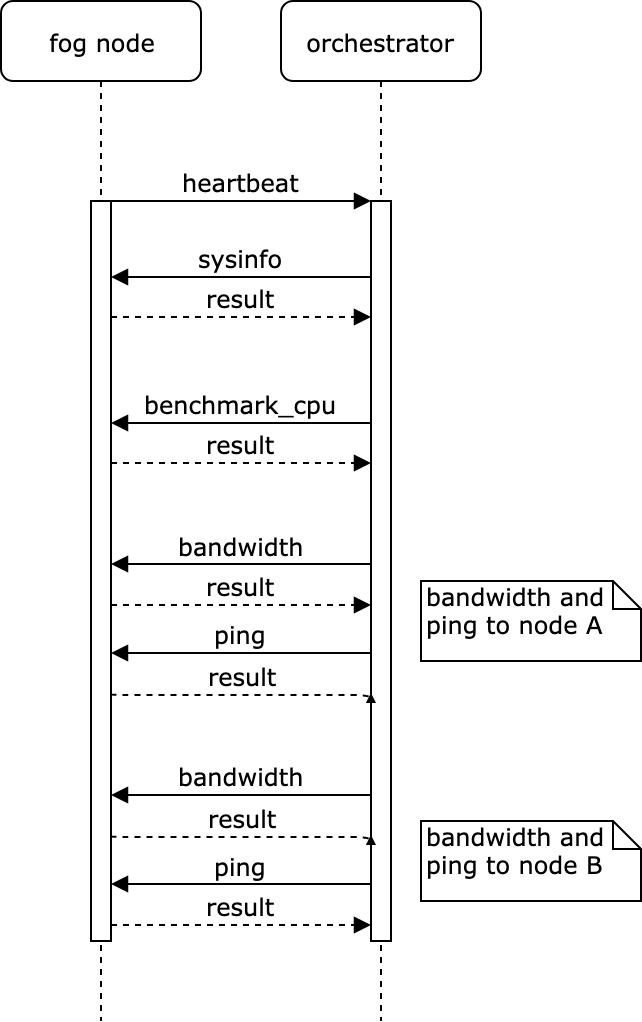
\includegraphics[width=0.5\textwidth]{orchestrator-initial-heartbeat}
    \caption{Sequence diagram of the orchestrator handling a new heartbeat}
    \label{fig:orchestrator-initial-heartbeat}
\end{figure}

After the Orchestrator has collected all required information about the node, it is added to the infrastructure and the \textit{Qos Scheduler} is run to (eventually) find a new optimal deployment.

\subsubsection*{Measuring bandwidth}
To measure the bandwidth a tool called \texttt{iperf3} was used first, which measures the transfer rate via \texttt{TCP}. However, these measured values could not be achieved in practice, since \texttt{HTTP} is used for message transmission between the modules. Because \texttt{HTTP} is build on top of \texttt{TCP}, it introduces additional protocol overhead and thus has a lower transfer rate than \texttt{TCP}. For this reason, \texttt{iperf3} was replaced by a measurement method using \texttt{HTTP}:

To measure the uplink from \textit{node A} to \textit{node B}, \textit{node A} sends a \texttt{HTTP POST} request to a predefined endpoint on \textit{node B}. The \texttt{HTTP body} initially contains \texttt{1MB} of data. After \textit{node B} has received the request, it responds with an empty body. \textit{Node A} can then calculate the \textit{transfer rate} by using the \textit{data size} and \textit{transfer time}.
If the response from node B is received fairly rapidly (less than 500ms), node A repeats the measurement with a larger data size to get a more accurate result.

\subsubsection*{Benchmarking CPU}
The algorithm uses the unit \textit{MIPS} to specify the speed of a CPU, respectively to specify the required CPU instructions of a module in order to calculate the execution time of a module on a node. However, \textit{MIPS} can't be read from the system like total RAM or amount of CPU cores. For this reason a CPU score is used instead. The Orchestrator calculates this score according to the following formula:
\[\textrm{CPU score} = \frac{10000}{\textrm{sysbench result [time in ms]}}\]

Thus, the lower the execution time of \texttt{sysbench}, the higher the CPU score. This score is used for the field \texttt{cpuMips} of a \texttt{FogNode} instance.

However, the field \texttt{requiredMips} of an \texttt{AppSoftwareModule} instance must also be set accordingly. To determine this value, the corresponding software module is executed on a node where we know the CPU score. Since we can measure the execution time on that node, the required value can be calculated as follows:
\[\textrm{required instructions} = \frac{\textrm{CPU score} \boldsymbol{\cdot} \textrm{execution time [ms]}}{1000}\]


\section{Using the QoS-Scheduler in the Orchestrator}

The output of the algorithm tells which module should be deployed on which node. In the example shown in table \ref{tab:deployment-strategy-example}, the algorithm has decided to distribute the three modules of the object detection application (see figure \ref{fig:object-detection-appmodules}) over two nodes (\textit{node A} and \textit{node B}).

\begin{table}[htb]
    \centering
    \begin{tabular}{|m{1.5cm}|m{4cm}|m{3.5cm}|}
        \hline
        \textbf{Order} & \textbf{Module} & \textbf{Executing node}\\
        \hline
        1 & \texttt{camera-controller} & node A\\
        \hline
        2 & \texttt{object-detector} & node B\\
        \hline
        3 & \texttt{image-viewer} & node A\\
        \hline
    \end{tabular}
    \caption{Sample deployment strategy for object detection application}
    \label{tab:deployment-strategy-example}
\end{table}

\subsection*{Node-RED Controller}

Every running Node-RED instance can be controlled via the \textit{Node-RED Admin API}\footnote{https://nodered.org/docs/api/admin/methods/}. In order to make use of it, the \texttt{NodeRedController} was implemented (see figure \ref{fig:orchestrator-classdisgram}). It is able to call all necessary API functions, so that the Orchestrator can control the Node-RED instances (create, update and delete flows in particular).

\subsection*{Flow database}
In a Node-RED context, each module is a Node-RED flow and is stored in a database. A node-RED flow in turn can be exported, saved and imported as JSON. However, in this architecture, nothing is manually exported and stored in a database. Instead, there is a dedicated Node-RED instance which serves exclusively as flow database and is not used for task execution. The Orchestrator can then query a specific flow from this instance via the \texttt{NodeRedController} by calling the method \texttt{getFlowByName(flowName)}.

The flow database is implemented in the class \texttt{NodeRedFlowDatabase} (see figure \ref{fig:orchestrator-classdisgram}).

\subsection*{Deploying flows}
The orchestrator fetches each flow from the database and deploys it to the node-RED instance running on the scheduled fog node. The orchestrator manages the flows on the nodes by using the \texttt{NodeRedController}. The process of deploying a deployment strategy (instance of \texttt{AppDeployment}) to the infrastructure is shown in figure \ref{fig:orchestrator-activitydiagram-deploy-flows}.

\begin{figure}[htb]
    \centering
    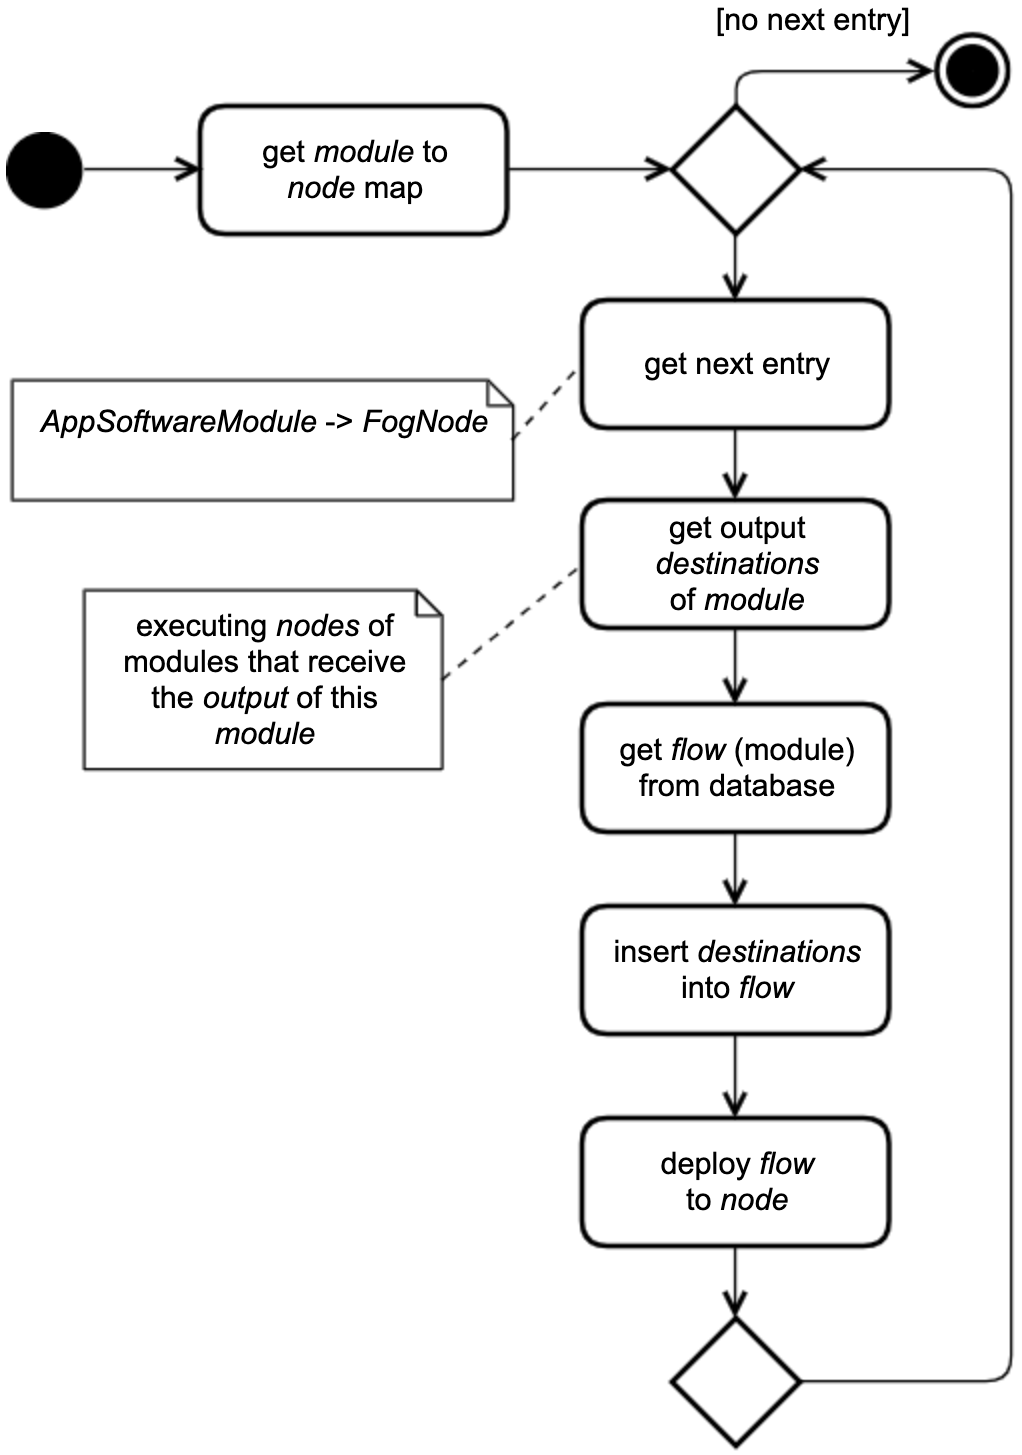
\includegraphics[width=0.7\textwidth]{orchestrator-activitydiagram-deploy-flows}
    \caption{Activity diagram for deploying an \texttt{AppDeployment} to a Node-RED infrastructure}
    \label{fig:orchestrator-activitydiagram-deploy-flows}
\end{figure}

\subsection*{Communication}
The communication between two application modules (Node-RED flows) is done by using the \textit{HTTP nodes} available in Node-RED. For instance, the module \texttt{object-detector} is accepting HTTP requests on the endpoint \texttt{/object-detection/object-detector} (module \textit{input}), so that the module \texttt{camera-controller} (the previous module in the loop) can send its \textit{output} via an \texttt{HTTP POST} request to that endpoint. However, \textit{node A} must know that the output of \texttt{camera-controller} must be send to \textit{node B}. To achieve this, the Orchestrator places the address of \textit{node B} in the \texttt{camera-controller} flow it got from the database before it deploys this flow to \textit{node A} (see figure \ref{fig:orchestrator-activitydiagram-deploy-flows}).

\section{Monitoring the current deployment strategy}

The Orchestrator must verify that the selected deployment strategy really meets the application requirements. Since the goal here is to get the result within a certain time, the last module in the loop must tell the Orchestrator how long it took to process the application loop. If the latency requirements could not be fulfilled, the Orchestrator must be able to identify the problem and react to the environmental changes.

To realize this, every application module attaches the current time \textit{before} and \textit{after} processing to the message object (or in other words: \textit{after} receiving the message, and \textit{before} sending a new message to the next module / node). From this values, the actual processing time on a node, as well as the transfer time for every message between two nodes can be calculated. Where the timestamps are taken and how these are used to calculate the individual processing and transfer times is illustrated in a timeline in figure \ref{fig:orchestrator-statistics-timeline}.

\begin{figure}[h]
    \centering
    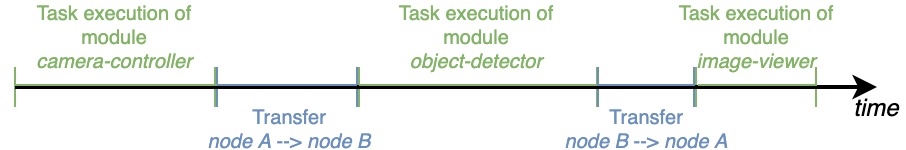
\includegraphics[width=1.0\textwidth]{orchestrator-statistics-timeline}
    \caption{Timeline for executing the loop of the object detection application}
    \label{fig:orchestrator-statistics-timeline}
\end{figure}

The calculates values are stored in a \texttt{statistics} object in the message and passed through to the next module. The last module in the loop sends this object to the Orchestrator via \texttt{MQTT}, which can then further analyze this object.

The \texttt{statistics} object contains two arrays:
\begin{enumerate}
    \item \texttt{transfers} for all message transfers between nodes
    \item \texttt{processes} for all task executions on the nodes
\end{enumerate}

An example is shown in listing \ref{lst:statistics}.

\lstinputlisting[language=json, caption=Sample statistics JSON object,label={lst:statistics}]{listings/statistics.json}

Not only the entire execution time of a loop can be extracted from that object, but also which part took how long. In the case of a downgrade of one network connection, it is possible to determine between which nodes the connection has downgraded. Since we know the \textit{size}, \textit{transfer time}, \textit{source node} and \textit{destination node}, the current bandwidth between those nodes can be calculated and the infrastructure can be updated accordingly. The Orchestrator can then run the algorithm with the updated values to see if there is a new optimal deployment.
    \chapter{Evaluation\label{cha:evaluation}}

In this chapter the Orchestrator introduced in chapter \ref{cha:orchestrator} is tested and evaluated. For this purpose an object detection application is used, which should be deployed to a given test infrastructure containing several devices.
In the first experiment the nodes join and leave the network one after the other.
The second experiment investigates how the system behaves upon network quality changes.
For both experiments it is examined which decisions the Orchestrator makes and what effect this decision has on the total latency of the application.







\section{Experimental setup}

\subsection{Infrastructure\label{sec:eval-infrastructure}}

\begin{figure}[htb]
    \centering
    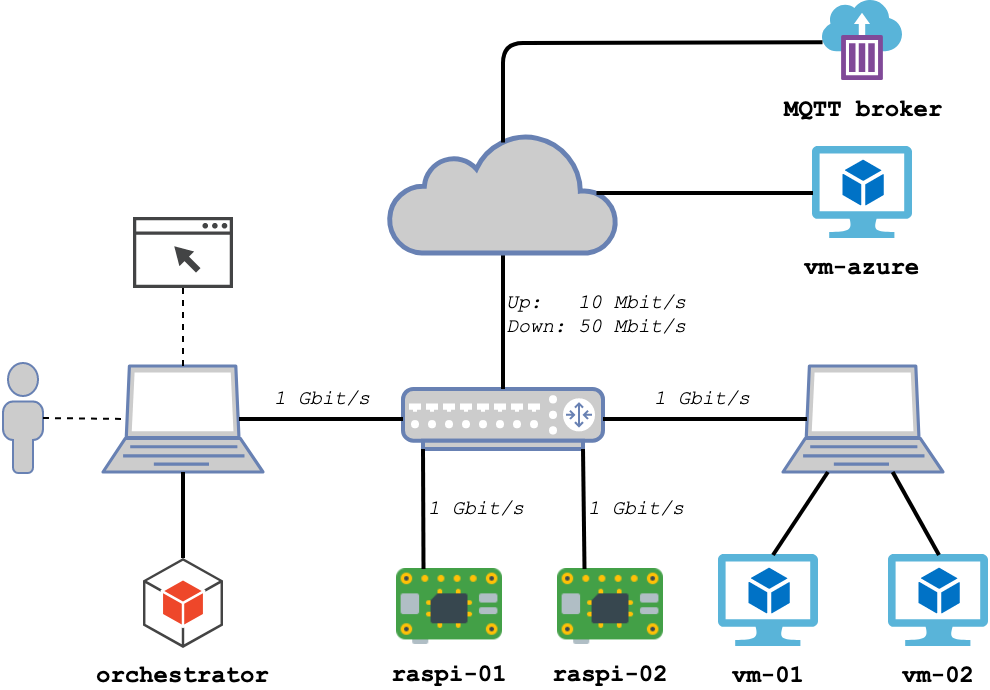
\includegraphics[width=0.85\textwidth]{evaluation-infrastructure}
    \caption{Test infrastructure for evaluation}
    \label{fig:evaluation-infrastructure}
\end{figure}

The test bed consists of the five nodes shown in figure \ref{fig:evaluation-infrastructure}. The hardware characteristics of the devices are shown in table \ref{tab:evaluation-devices}. The three virtual machines run Debian 10, the two Raspberry Pis run Raspbian 10. All nodes have \texttt{Docker version 19.03.2} installed. Another device on the local network runs the Orchestrator and a web browser which is used to access the \textit{Object Detection Web Application}. Communication between the nodes and the Orchestrator is done via an MQTT broker running in the Azure Cloud.

\begin{table}[htb]
    \centering
    \begin{tabular}{|l|l|l|l|l|l|}
    \hline
        \textbf{Node} & \textbf{Device Type} & \textbf{CPU} & \textbf{RAM} \\
         \hline
         \texttt{raspi-01} & Raspberry Pi 3B+ & ARM Cortex-A53 1.4 GHz, 4 cores & 1 GB\\
         \hline
         \texttt{raspi-02} & Raspberry Pi 4B & ARM Cortex-A72 1.5 GHz, 4 cores & 4 GB\\
         \hline
         \texttt{vm-01} & Hyper-V VM & Intel i7-8550U 1.8 GHz, 2 vCPUs & 2 GB\\
         \hline
         \texttt{vm-02} & Hyper-V VM & Intel i7-8550U 1.8 GHz, 4 vCPUs & 4 GB\\
         \hline
         \texttt{vm-azure} & Azure VM \texttt{F4s\_v2} & Intel Xeon 2.7 GHz, 4 vCPUs & 8 GB\\
         \hline
    \end{tabular}
    \caption{Hardware characteristics of test devices used for evaluation}
    \label{tab:evaluation-devices}
\end{table}

\subsection{Application\label{sec:eval-application}}

\begin{figure}[htb]
    \centering
    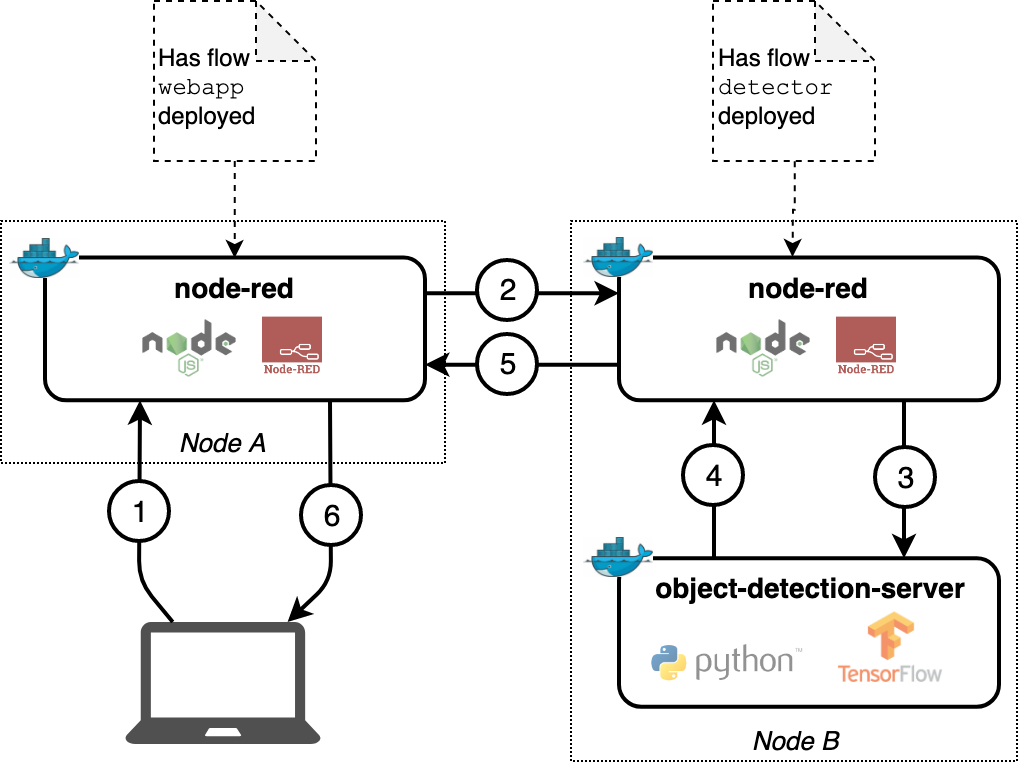
\includegraphics[width=0.85\textwidth]{evaluation-application}
    \caption{System architecture of Object Detection Web Application}
    \label{fig:evaluation-object-detection-application}
\end{figure}

The \textit{Object Detection Web Application} consists of the two modules \texttt{webapp} and \texttt{detector} as illustrated in figure \ref{fig:evaluation-object-detection-application}. A screenshot of the web application is shown in figure \ref{fig:object-detection-webapp-screenshot}.\\

In the first step, a user sends an image for object detection to the \texttt{webapp} module which is deployed as a Node-RED flow on \texttt{Node A}. This module should always be deployed on the same node and not be moved so that the web application is always available at the same address. The user calls the web application from that fixed node and he does not care which node actually executes the object detection task. The module \texttt{webapp} forwards the image to the module \texttt{detector} for object detection which is deployed on another node (\texttt{Node B}). This node can vary and is chosen by the Orchestrator. If a new node is selected by the Orchestrator, then the flow \texttt{webapp} on \texttt{Node A} will be updated so that subsequent requests are forwarded to the new node.\\

The object detection engine can not be executed as a regular Node-RED flow since Node-RED handles JavaScript functions only and the engine requires Python. Even if Node-RED could execute Python code (there are extensions enabling this) the execution of the object detection engine in Node-RED would not be efficient because the engine would have to be initialized every time a new object detection request arrives. However, the engine has a certain initialization time to load the detection graph. Therefore it is more efficient to initialize the engine only once at the beginning so that the following object detection tasks can be executed without additional initialization time. Because Node-RED can not initialize and hold Python objects, a separate docker container is used for this purpose. The flow \texttt{detector} sends an HTTP request containing the undetected image to the \texttt{object-detection-server} running on the same node. The server responds with the detected image which the \texttt{detector} then sends back to the \texttt{webapp} module.

The following three constraints are defined for the experiment:
\begin{enumerate}
    \item The flow \texttt{webapp} must be deployed on \texttt{raspi-01} because this is the only node known to the user
    \item The flow \texttt{detector} needs an \texttt{object-detection-server} docker container running on the same node which is the case for all nodes except for \texttt{raspi-01}
    \item The detected image must be available within 5 seconds
\end{enumerate}








\section{Preparing the Orchestrator\label{sec:eval-preparing-the-orchestrator}}

For evaluating the Orchestrator we need nodes with different CPU performance(s?).
However, one vCPU in \texttt{vm-01} is equally fast as in \texttt{vm-02} because they both run on the same host.
Since the object detection engine uses only one core, the execution time on these two nodes is approximately the same, although \texttt{vm-01} has two cores and \texttt{vm-02} has four cores. For this reason, the docker containers on \texttt{vm-01} run with the additional option \texttt{---cpus="0.5"} which limits the available CPU resources a container can use to a half vCPU.

\subsection{Possible deployment strategies and their respective latencies\label{sec:eval-possible-deployments}}
To find the real execution times of all possible deployment strategies, the application was deployed to the infrastructure without using the Orchestrator.
The module \texttt{webapp} was always deployed on node \texttt{raspi-01} while the module \texttt{detector} was switched through the remaining nodes.
The object detection application was executed 10 times on each deployment strategy by using a 1,383 KB sized image.
The mean values for \textit{total latency}, \textit{processing time} and \textit{transfer time} were calculated thereafter. These are compared in figure \ref{fig:evaluation-total-latency-without-orchestrator}.

\begin{figure}[h!]
    \centering
    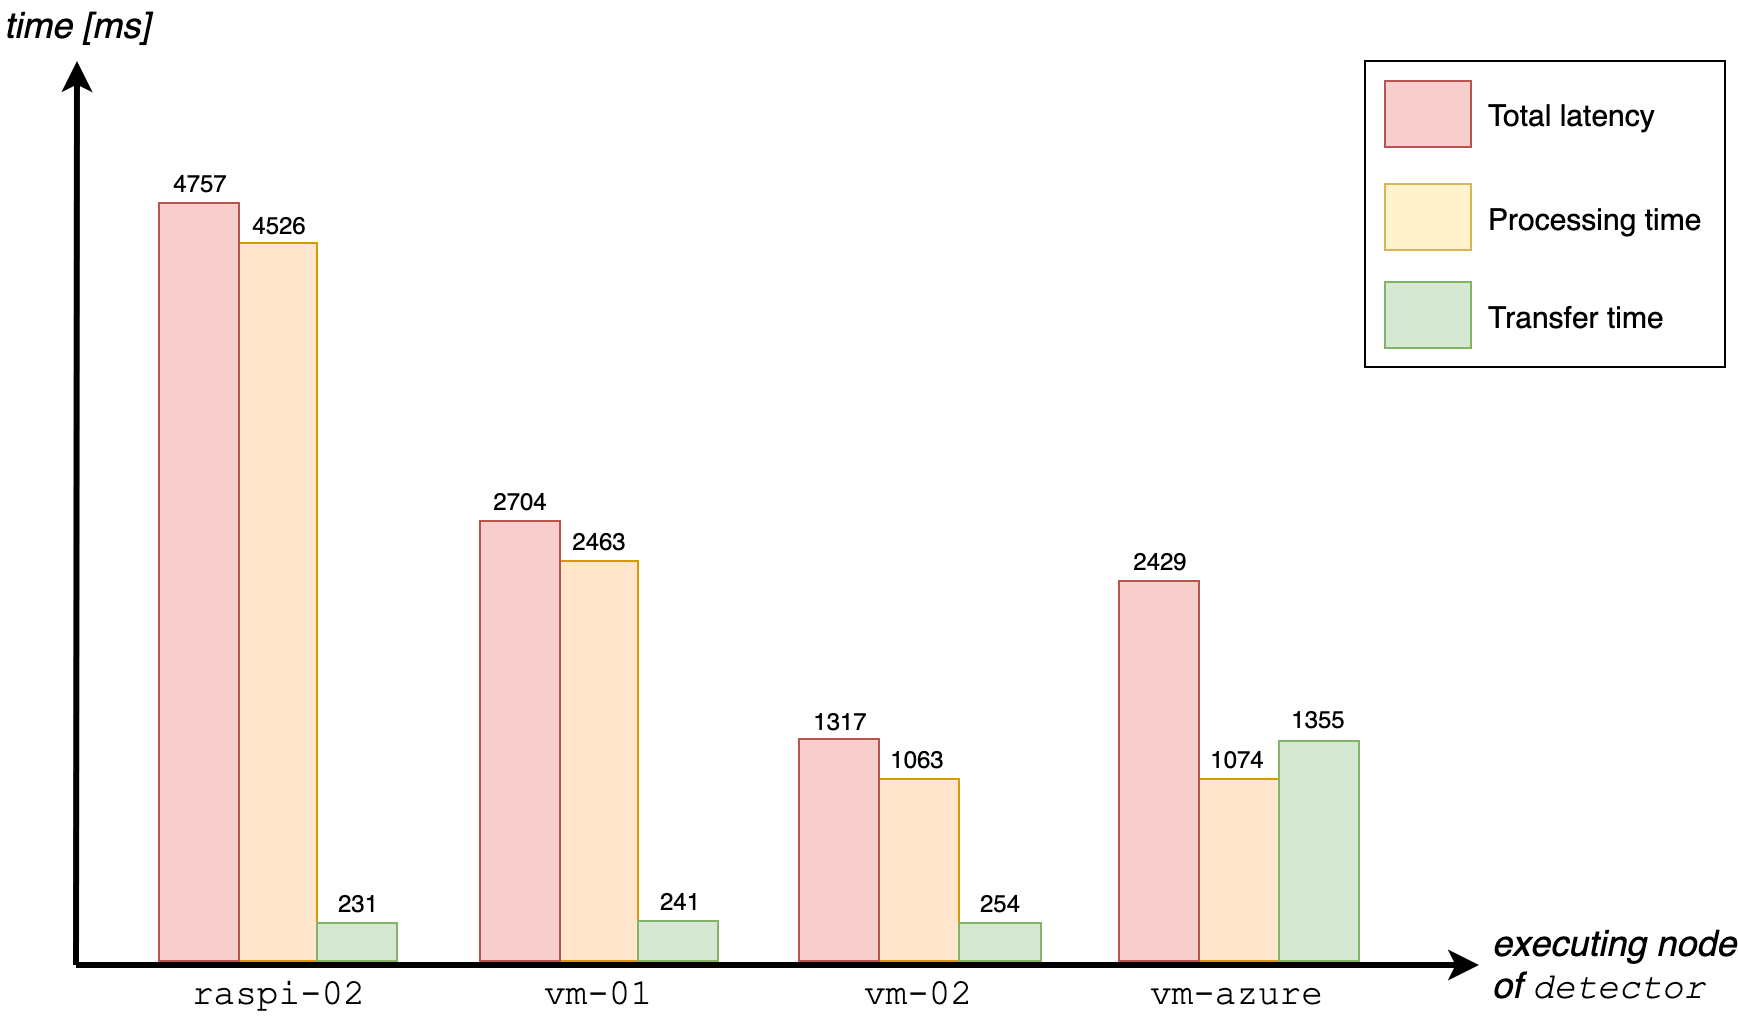
\includegraphics[width=1.0\textwidth]{evaluation-total-latency-without-orchestrator}
    \caption{Total latencies, processing and transfer times of the object detection application regarding the placement of module \texttt{detector}}
    \label{fig:evaluation-total-latency-without-orchestrator}
\end{figure}

Based on the measurement results, a prioritization of all possible deployments was created where deployments with a lower latency were preferred (see table \ref{tab:deployment-strategies-prios}).
\begin{table}[h!tb]
    \centering
    \begin{tabular}{|l|l|l|l|l|l|}
    \hline
        \textbf{Priority} & \textbf{Placement of \texttt{webapp}} & \textbf{Placement of \texttt{detector}} & \textbf{Latency} \\
         \hline
         \texttt{1} & \texttt{raspi-01} & \texttt{vm-02} & 1,317 ms\\
         \hline
         \texttt{2} & \texttt{raspi-01} & \texttt{vm-azure} & 2,429 ms\\
         \hline
         \texttt{3} & \texttt{raspi-01} & \texttt{vm-01} & 2,704 ms\\
         \hline
         \texttt{4} & \texttt{raspi-01} & \texttt{raspi-02} & 4,757 ms\\
         \hline
    \end{tabular}
    \caption{Possible deployment strategies \textcolor{red}{\textbf{for (of?)}} object detection application}
    \label{tab:deployment-strategies-prios}
\end{table}

\subsection{Defining the Application\label{sec:eval-defining-application}}

Although the Orchestrator handles the infrastructure dynamically, an application must be defined. 
Therefore, an \texttt{Application} object is created during the initialization of the Orchestrator.
It contains all modules, loops and messages of the object detection application described in section \ref{sec:eval-application}.

\subsubsection*{Setting required RAM and disk storage}
The fields \texttt{requiredRam} and \texttt{requiredStorage} of the two modules \texttt{webapp} and \texttt{detector} are set to \texttt{0} because both Node-RED flows are relatively small and thus consume neither significant RAM nor storage.
Although the \texttt{object-detection-server} container requires 1GB RAM, this memory is not allocated/released by deploying/removing the flow to/from Node-RED because the container runs even if the Node-RED flow is not deployed on a node.
Furthermore, the container does not require any additional disk storage while running the engine.

\subsubsection*{Setting required hardware modules}
The field \texttt{requiredHardwareModules} of the module \texttt{webapp} contains one string: \texttt{"CAMERA"}.
The \texttt{node-red} docker container on \texttt{raspi-01} is started with the additional option \texttt{-e CONNECTED\_HARDWARE=["CAMERA"]} so that \texttt{webapp} can only be deployed \textcolor{red}{\textbf{on (to?)}} \texttt{raspi-01}. The same approach is used for the module \texttt{detector}, but here the string \texttt{"OD-DOCKER-CONTAINER"} is used and passed to the docker container on the remaining nodes instead.

\subsubsection*{Setting required instructions}
The field \texttt{requiredMi} of the module \texttt{webapp} is set to \texttt{0} because the Node-RED flow simply forwards messages and therefore does not require any significant CPU power.
However, CPU resources consumed by the module \texttt{detector} are substantial.
Since the Orchestrator uses a CPU score instead of MIPS, the value for \texttt{requiredMi} has to be calculated using the formula introduced in section \ref{sec:benchmark-cpu}.
Values for \textit{CPU score} and \textit{execution time} are taken from \texttt{vm-02}, which are \textit{11661} and \textit{1317 ms}, respectively.
Therefore:
\[\textrm{\texttt{requiredMi\textsubscript{detector}}} = \textrm{CPU score} \boldsymbol{\cdot} \frac{\textrm{execution time [ms]}}{1,000 \textrm{ [ms]}} = 11,661 \boldsymbol{\cdot} \frac{1,317}{1,000} = 15,357\]

\subsubsection*{Setting the loop and messages}
The application has exactly one loop (instance of \texttt{AppLoop}) where the field \texttt{modules} is populated with a list containing three elements in the following order:
\texttt{"webapp"}, \texttt{"detector"}, \texttt{"webapp"}.
The field \texttt{maxLatency} is set to \texttt{5000}.

Furthermore, the application contains two messages (instaces of \texttt{AppMessage}).
The first one contains the original image, which in this case has a file size of 1,383 KB. Therefore, the fields \texttt{contentType} and \texttt{dataPerMessage} are set to \texttt{"IMAGE\_UNDETECTED"} and  \texttt{1383}, respectively. This is the input message to the module \texttt{detector}.
The second message contains the detected image, which has a file size of 142 KB. Therefore, the fields are set to \texttt{"IMAGE\_DETECTED"} and \texttt{142}, respectively. This is the output message of the module \texttt{detector}.









\section{Experiment 1: Consistent network quality\label{sec:eval-exp-1}}

In this experiment, the nodes were started in the following order:
\begin{enumerate}
    \item \texttt{raspi-01}
    \item \texttt{raspi-02}
    \item \texttt{vm-01}
    \item \texttt{vm-azure}
    \item \texttt{vm-02}
\end{enumerate}
This order allows to deploy the deployment strategy of lowest priority (priority four) in step two, while with each following step a strategy of higher priority is possible (see table \ref{tab:deployment-strategies-prios}).

It was expected that the Orchestrator finds no valid deployment in step one because here only \texttt{raspi-01} is online which is not able to execute the module \texttt{detector}.
Another expectation was that the Orchestrator deploys the module \texttt{webapp} to \texttt{raspi-01} and \texttt{detector} to \texttt{raspi-02} in the second step and then moves the \texttt{detector} to \texttt{vm-01}, \texttt{vm-azure} and finally to \texttt{vm-02} in the subsequent steps, while \texttt{webapp} remains on \texttt{raspi-01}.

\subsection*{Results}

\begin{figure}[htb]
    \centering
    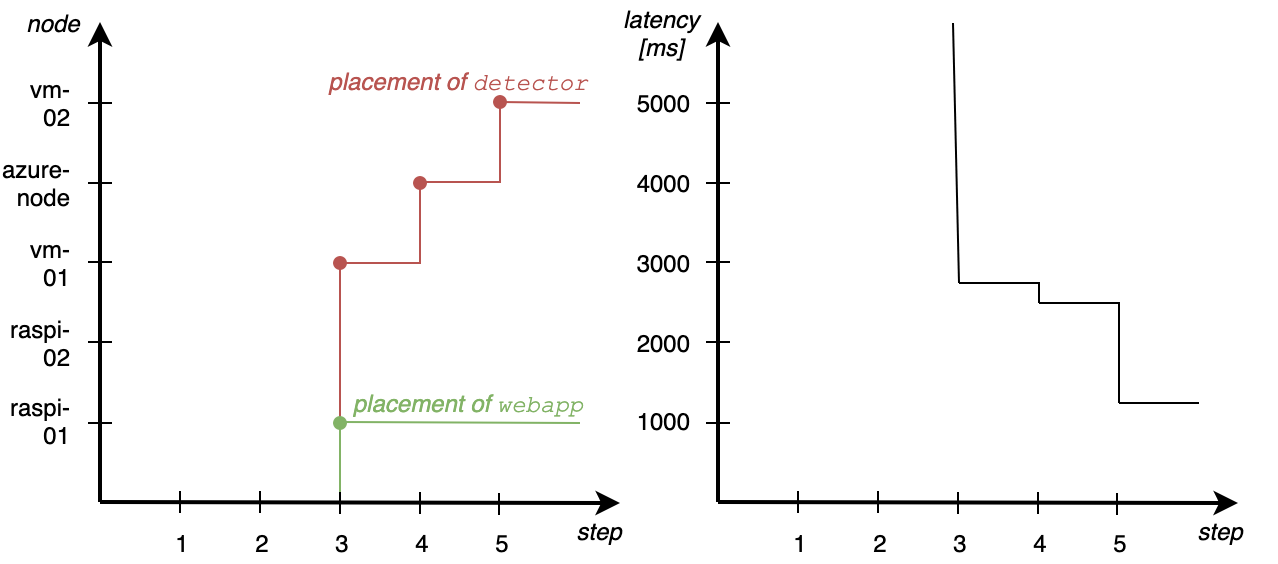
\includegraphics[width=1.0\textwidth]{evaluation-exp1-result}
    \caption{Result of Experiment 1: Orchestrator's decisions and their impact on total latency}
    \label{fig:evaluation-exp1-results}
\end{figure}

The Orchestrator's decisions are depicted in figure \ref{fig:evaluation-exp1-results}. As we can see, the Orchestrator behaved slightly different than expected. The \texttt{detector} was expected to be deployed to \texttt{raspi-02} in the second step. However, this did not happen. Instead, no possible deployment was found. In steps 1, 3, 4 and 5, however, the Orchestrator made the expected decisions and the latency is continuously minimized from step 3 onwards.

Moreover, it was examined how the Orchestrator behaves when a node leaves the network.
If a node that has \textit{no} module deployed leaves the network, the Orchestrator detects this and removes it from the infrastructure. The deployment strategy remains unchanged as it should be.
If a node that \textit{has} a module deployed leaves the network, the Orchestrator detects this and removes it from the infrastructure first before it then finds and applies the next best possible deployment strategy (next best deployment strategy is the one of highest priority in the updated infrastructure).
This complies with the desired behaviour.

\subsection*{Investigation of the Orchestrator's incorrect decision\label{sec:eval-investigation-cpu}}

The reason for the wrong decision in step two is that the execution time of module \texttt{detector} on node \texttt{raspi-02} calculated by the Orchestrator is incorrect.
The field \texttt{cpuMips} of the \texttt{FogNode} object representing this node has the value 973.
This value is the CPU score returned by the \texttt{benchmark\_cpu} command which the Orchestrator executed on the node after the first heartbeat has been received (see section \ref{sec:handling-new-fog-nodes} and \ref{sec:benchmark-cpu} in particular).
To calculate the execution time of module \textit{M} on node \textit{N}, the Orchestrator uses \texttt{cpuMips} of \textit{N} and \texttt{requiredMi} of \textit{M}.
While preparing the Orchestrator in section \ref{sec:eval-preparing-the-orchestrator}, we set \texttt{requiredMi\textsubscript{detector}} to 15,357. Thus, the execution time is calculated as follows:

\[\textrm{execution time [ms]} = \frac{\textrm{\texttt{requiredMi}}}{\textrm{\texttt{cpuMips}}}\ \boldsymbol{\cdot} 1,000 = \frac{15,357}{973}\ \boldsymbol{\cdot} 1,000 = 15,783 \textrm{ [ms]}\]

The calculated execution time is approximately 3.5 times greater than actual execution time of 4,526 milliseconds (see figure \ref{fig:evaluation-total-latency-without-orchestrator}).
Furthermore, it is greater than 5,000 milliseconds, which is the \texttt{maxLatency} of the opject detection loop. 
Therefore, the Orchestrator finds no valid deployment strategy.

The \texttt{benchmark\_cpu} command internally uses the CPU benchmarking tool \texttt{sysbench} which searches for all prime numbers between 1 and a certain upper limit (2000 in this case) and returns the time needed to execute this task.
Apparently, this time cannot be used to deduce the execution time of other types of tasks like object detection.
To further investigate this, the simple JavaScript function shown in listing \ref{lst:simple-javascript-function} was executed in Node-RED on \texttt{raspi-02} and \texttt{vm-02} while no other CPU intensive processes were running.

\begin{lstlisting}[language=JavaScript,numbers=none,caption={JavaScript function which executes simple mathematical tasks while measuring the total execution time},label=lst:simple-javascript-function]
const timeStart = new Date();
let result = 0;
for (let i=0; i < Math.pow(10,7); i++) {
    result = result + i;
}
const timeEnd = new Date();
const time = timeEnd - timeStart;
\end{lstlisting}

The field \texttt{time} of that function contains the execution time in milliseconds which is approximately 2,500 on \texttt{vm-02} and 7,500 on \texttt{raspi-02}, respectively. 
Thus, the execution of the function is about \textit{3 times faster} on \texttt{vm-02} than on \texttt{raspi-02}, even though the CPU score of \texttt{vm-02} (11,848) is about \textit{12 times greater} than the score of \texttt{raspi-02} (973).
What's more, the object detection task takes about 1,063 milliseconds on \texttt{vm-02} and 4,757 milliseconds on \texttt{raspi-02}, which is a \textit{4,2-fold difference} (see figure \ref{fig:evaluation-total-latency-without-orchestrator}). A correlation between the execution times of different tasks on various nodes can therefore not be recognized.

However, there might be a correlation between CPUs that share the same architecture, but this is not the case either:
Executing the function shown in listing \ref{lst:simple-javascript-function} takes about 17,800 milliseconds on \texttt{raspi-01}, which is \textit{2.37 times slower} than on \texttt{raspi-02}, although the CPU score of \texttt{raspi-01} (612) is only \textit{1.59 times smaller} than on \texttt{raspi-02}. Both nodes own a CPU of type \texttt{arm}.\\

In conclusion, the execution time of a given task cannot be used as the basis to compare CPU performances of different devices.
There seem to be a number of relevant factors affecting the execution time of a task, but this goes beyond the scope of this work.




\section{Experiment 2: Volatile network conditions}

In this experiment, the three nodes \texttt{raspi-01}, \texttt{vm-01} and \texttt{vm-azure} were online.
Under these circumstances, deployment strategy of \textit{priority two} allows the lowest latency (see table \ref{tab:deployment-strategies-prios}).
Here, the \texttt{detector} module is deployed on \texttt{vm-azure}.
In further course, the router's Internet connection was utilized by other hosts in the network which are not part of the Fog infrastructure.
After a certain period, the bandwidth was freed again.

It was expected that the Orchestrator moves the \texttt{detector} module from \texttt{vm-azure} to \texttt{vm-01} as soon as the Internet connection is utilized that much that the maximum latency of 5,000 milliseconds cannot be guaranteed.
After the full bandwidth is available again, the \texttt{detector} should be moved back to \texttt{vm-azure}.


\subsection*{Results}

\begin{figure}[htb]
    \centering
    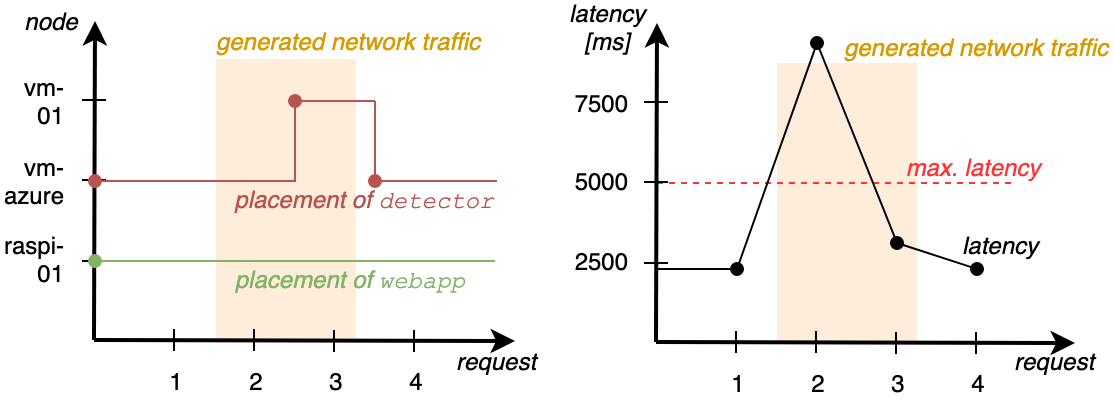
\includegraphics[width=1.0\textwidth]{evaluation-exp2-result}
    \caption{Result of Experiment 2: Orchestrator's decisions and their impact on total latency}
    \label{fig:evaluation-exp2-results}
\end{figure}

The Orchestrator's decisions are depicted in figure \ref{fig:evaluation-exp2-results}. 
Initially, he applied deployment strategy of priority two as expected.
The object detection task in request one was finished after 2,370 milliseconds, while the \texttt{detector} was executed on \texttt{vm-azure}.

Between request one and two, network traffic between a host in the local network and another host on the Internet was generated.
Both hosts were not part of the Fog infrastructure, but they did utilize the same Internet connection that was used for transferring the original image from \texttt{webapp} (deployed on \texttt{raspi-01}) to \texttt{detector} (deployed on \texttt{vm-azure}) as well.
That's why the maximum latency requirement of 5,000 milliseconds could not be met in request two.
Although the object detection task on \texttt{vm-azure} took approximately the same time in both requests, the time for transferring the original image (1,382 KB) took 7,641 milliseconds instead of 1,192 milliseconds in request one, to that the total latency added up to 8,921 milliseconds.

The Orchestrator recognized this by evaluating the \texttt{statistics} object (see listing \ref{lst:statistics}) introduced in section \ref{sec:orchestrator-monitoring-deployment-strategy}.
Based on the image size and transfer time, he calculated the actual bandwidth between both nodes, which is \textit{1.48 Mbit/s} in this case.
The respective \texttt{NetworkUplink} object was updated and the scheduling algorithm was executed to find a new optimal deployment strategy.
This is what happened between request two and three, before the \texttt{detector} was moved to \texttt{vm-01}.
As you can see, the latency requirement was fulfilled in request three, although the total latency of 2,671 milliseconds is a bit higher than in request one.

As said before, the scheduling algorithm was triggered during the evaluation of the \texttt{statistics} object in this case.
However, the algorithm is executed in a predefined interval as well.
Since the uplinks are also remeasured in a predefined interval, the scheduling algorithm might find a new optimal deployment strategy.
This is what happened between request three and four:
The network traffic generation has been stopped and the uplink between \texttt{raspi-01} and \texttt{vm-azure} has been remeasured.
The updated bandwidth was taken into account during the subsequent execution of the scheduling algorithm, so that the Orchestrator switched back to the deployment strategy of priority two which led to a lower latency in request four.

It should be added that there might be a new optimal deployment in case of a downgrade of an uplink, even though the new optimal deployment might have a higher latency than the previous one.
This could be the case if an uplink downgrades that is used in the current deployment strategy.
Nevertheless, the Orchestrator always applies the deployment strategy which allows the lowest latency to the best of his knowledge.



\section{Discussion}

TODO

- CPU: Intel -> gut vergleichbar; ARM -> nicht gut vergleichbar
alternative methode: test ausführung von modules und sich die zeit merken

problem: input size --> auch hier wären erfahrungswerte besser

Problem: webapp hat zwei input und zwei output types

problem: netzwerkmessungen bei vielen nodes

    \clearpage
\printbibliography
\clearpage

\listoffigures



\listoftables
\lstlistoflistings

    \chapter{UML diagrams\label{cha:algorithm-UML-diagrams}}

\begin{figure}[htb]
    \centering
    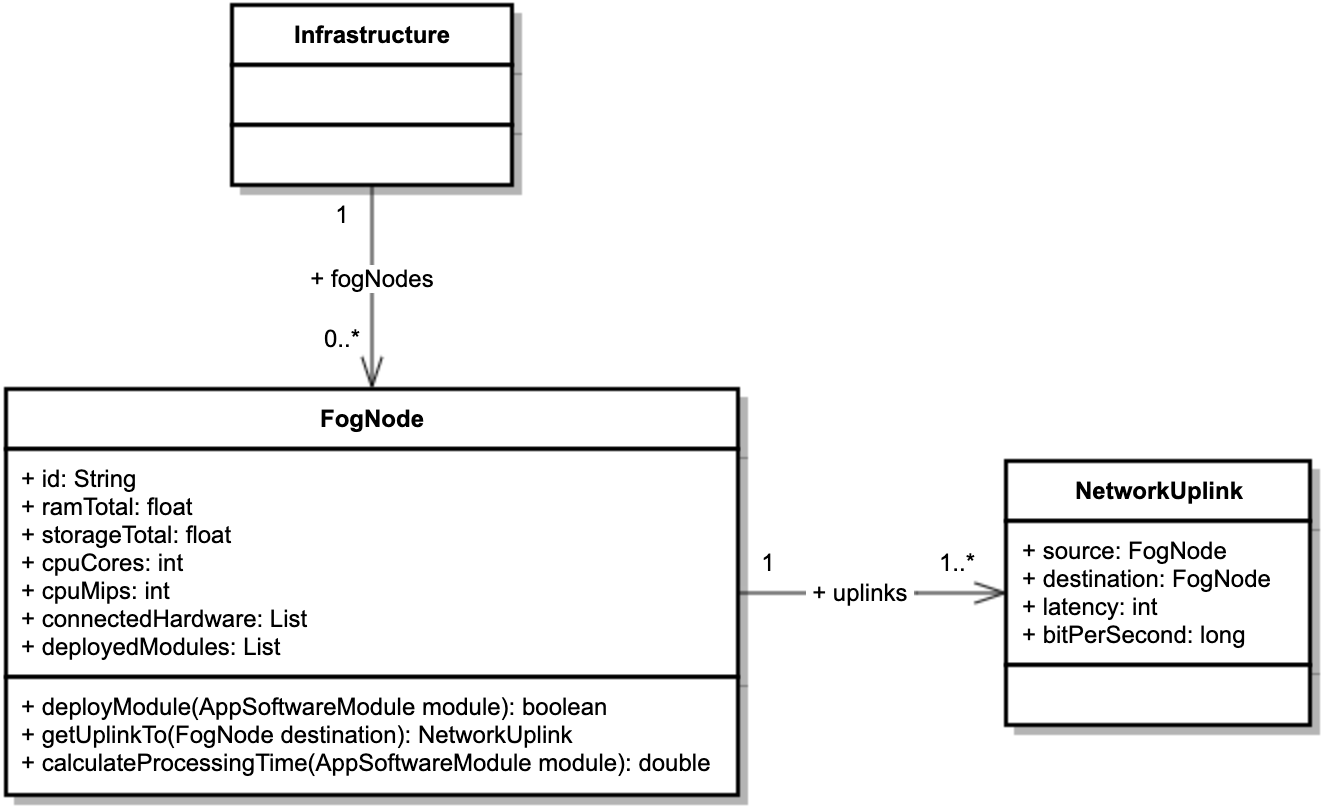
\includegraphics[width=1.0\textwidth]{algorithm-classdiagram-infrastructure}
    \caption{Class diagram of \texttt{Infrastructure}}
    \label{fig:classdiagram-infrastructure}
\end{figure}

\begin{figure}[htb]
    \centering
    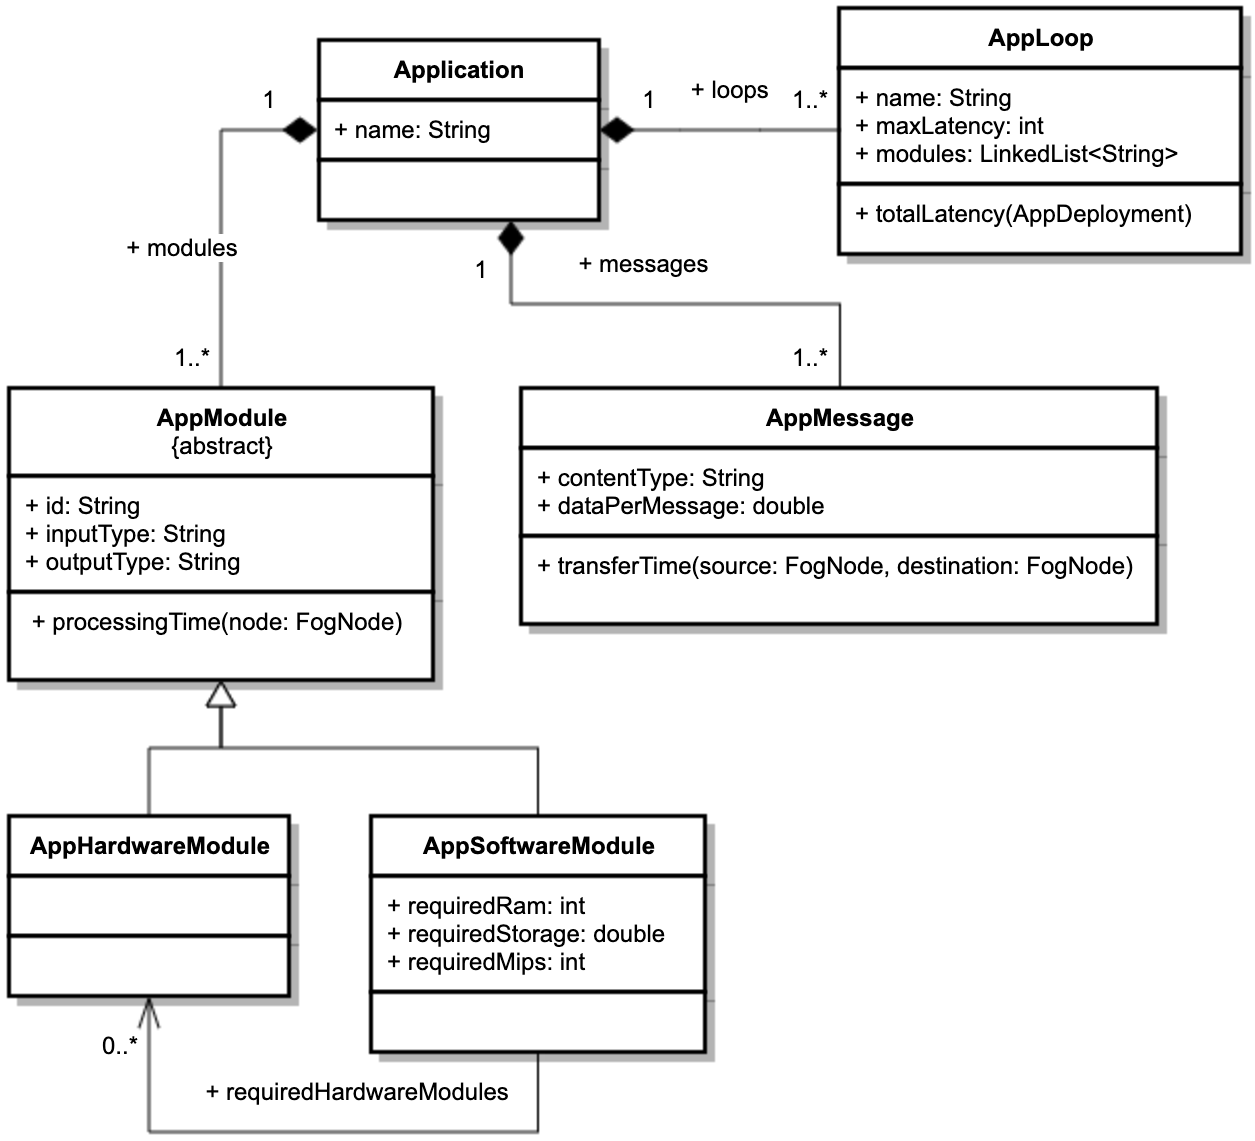
\includegraphics[width=1.0\textwidth]{algorithm-classdiagram-application}
    \caption{Class diagram of \texttt{Application}; TODO: REMOVE processingTime from AppModule}
    \label{fig:classdiagram-application}
\end{figure}

\begin{figure}[htb]
    \centering
    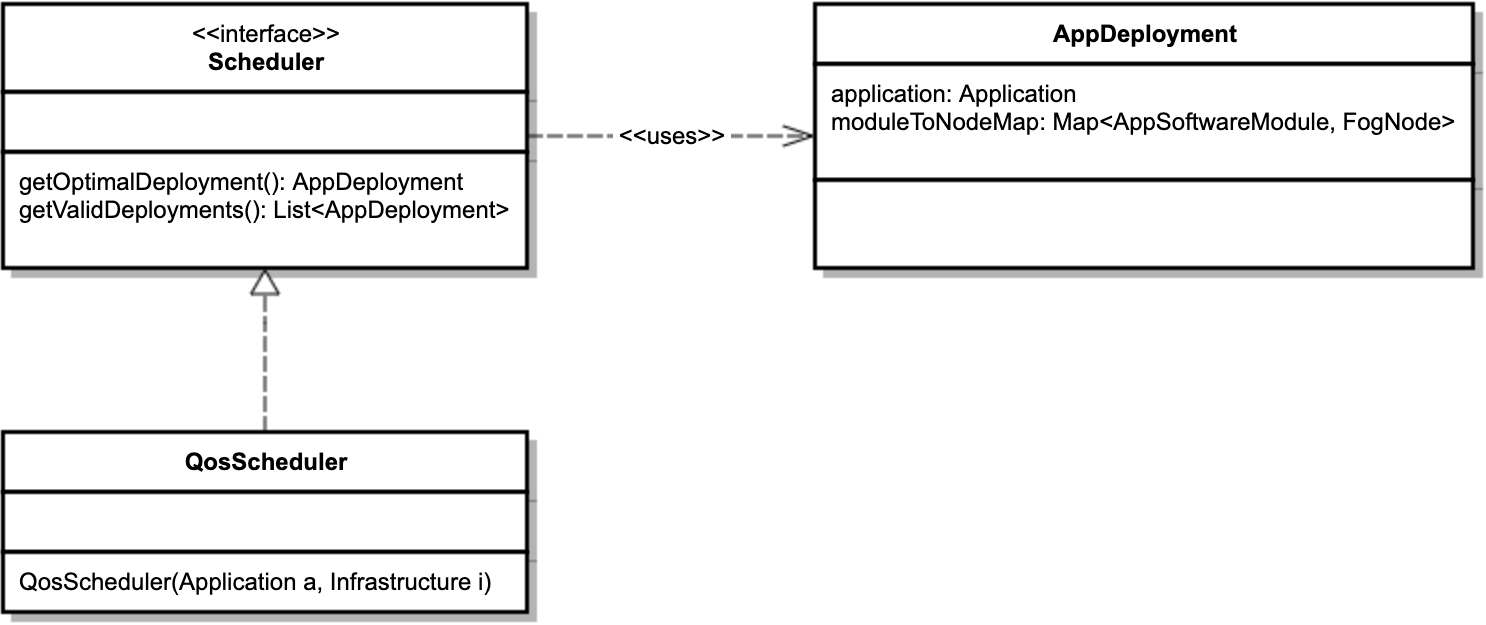
\includegraphics[width=1.0\textwidth]{algorithm-classdiagram-qosscheduler}
    \caption{Class diagram of \texttt{QosScheduler}}
    \label{fig:classdiagram-qosscheduler}
\end{figure}

\begin{figure}[htb]
    \centering
    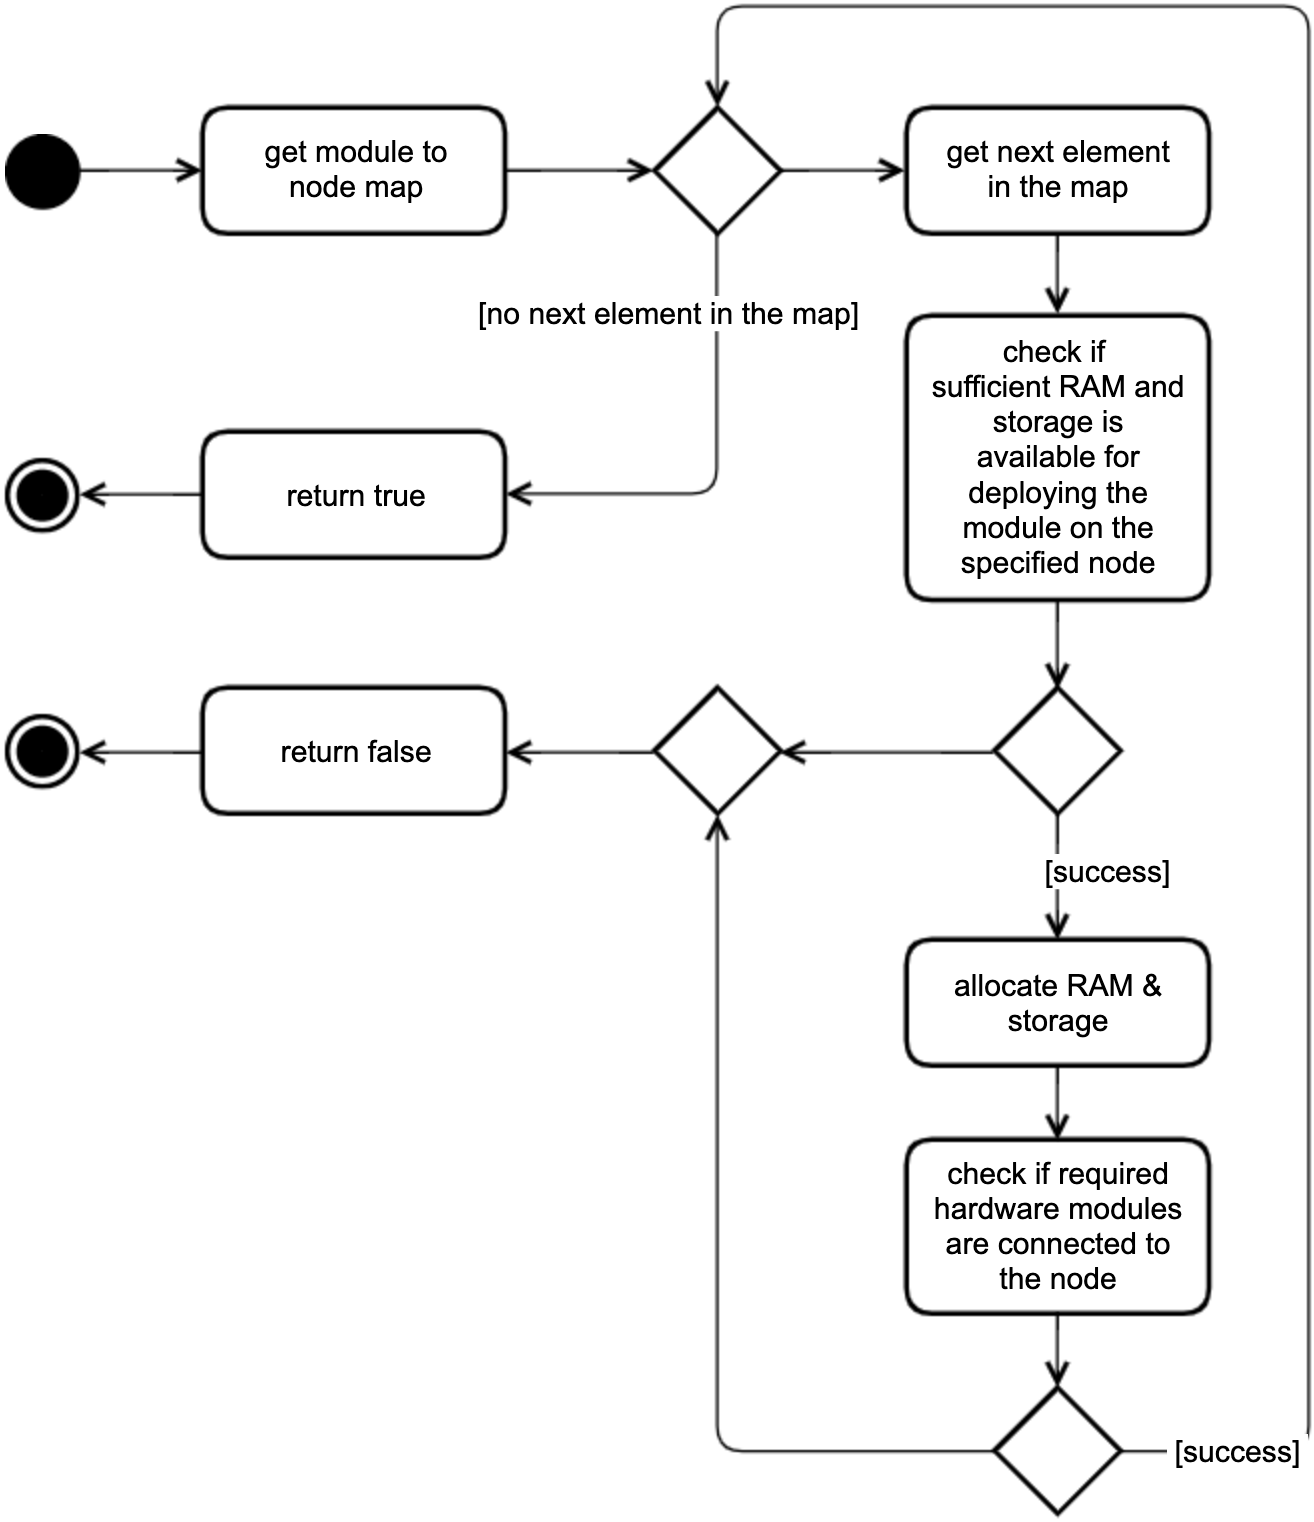
\includegraphics[width=0.9\textwidth]{algorithm-activitydiagram-hardware}
    \caption{Activity diagram for validating hardware requirements}
    \label{fig:algorithm-activitydiagram-hardware}
\end{figure}


\begin{figure}[htb]
    \centering
    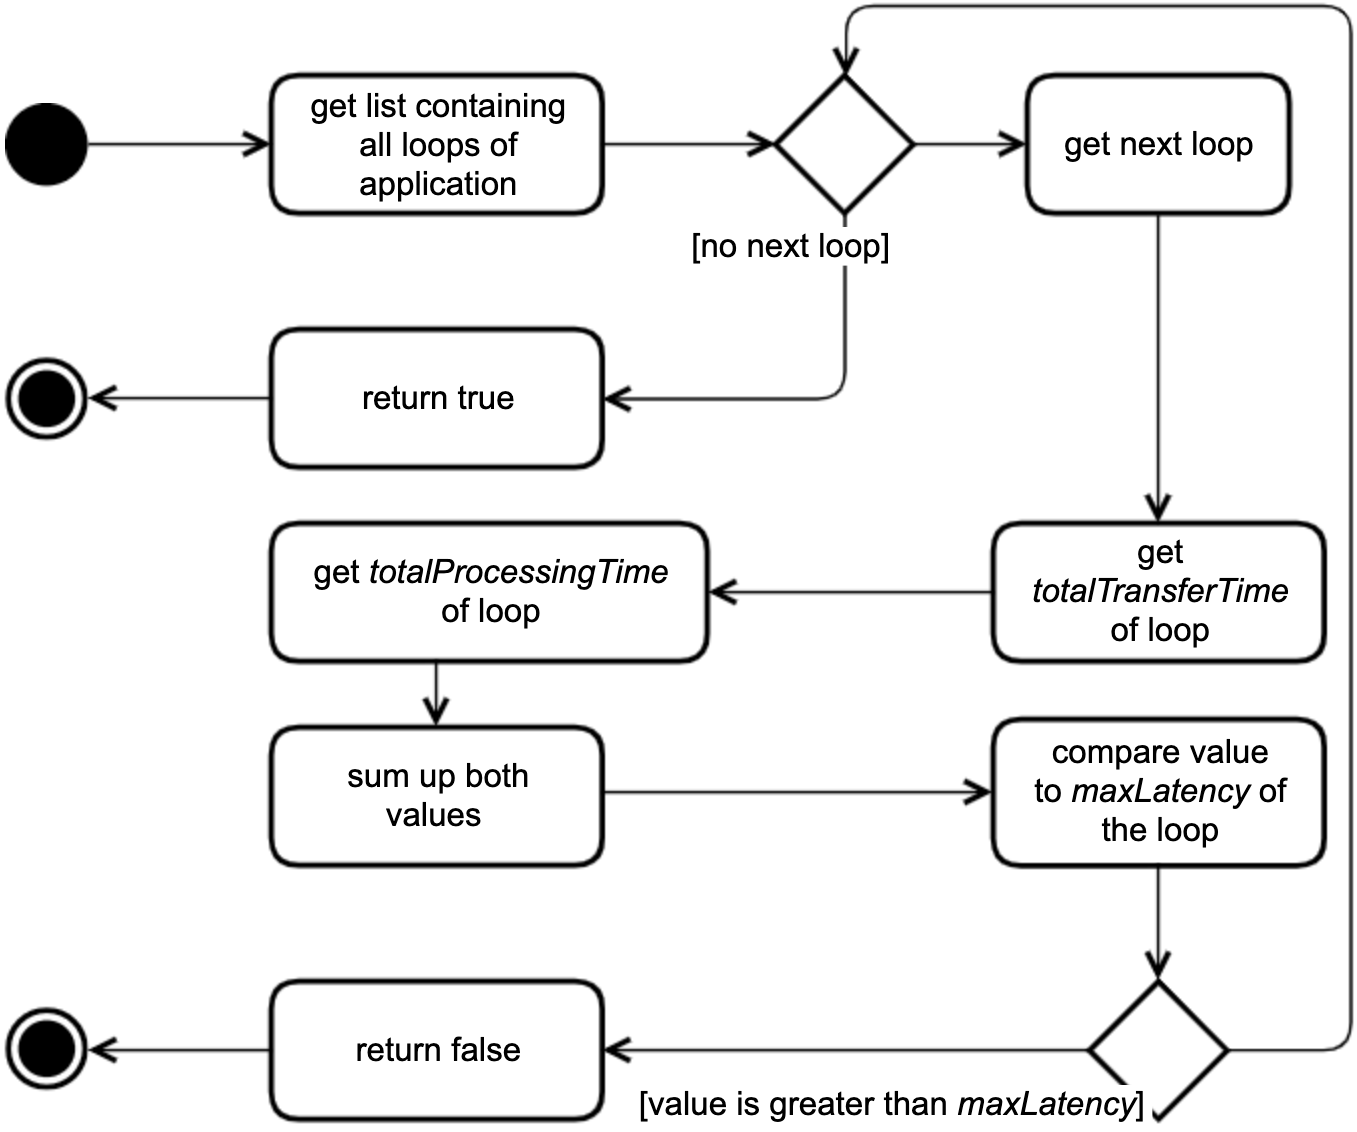
\includegraphics[width=0.9\textwidth]{algorithm-activitydiagram-latency}
    \caption{Activity diagram for validating latency requirements}
    \label{fig:algorithm-activitydiagram-latency}
\end{figure}

\begin{figure}[htb]
    \centering
    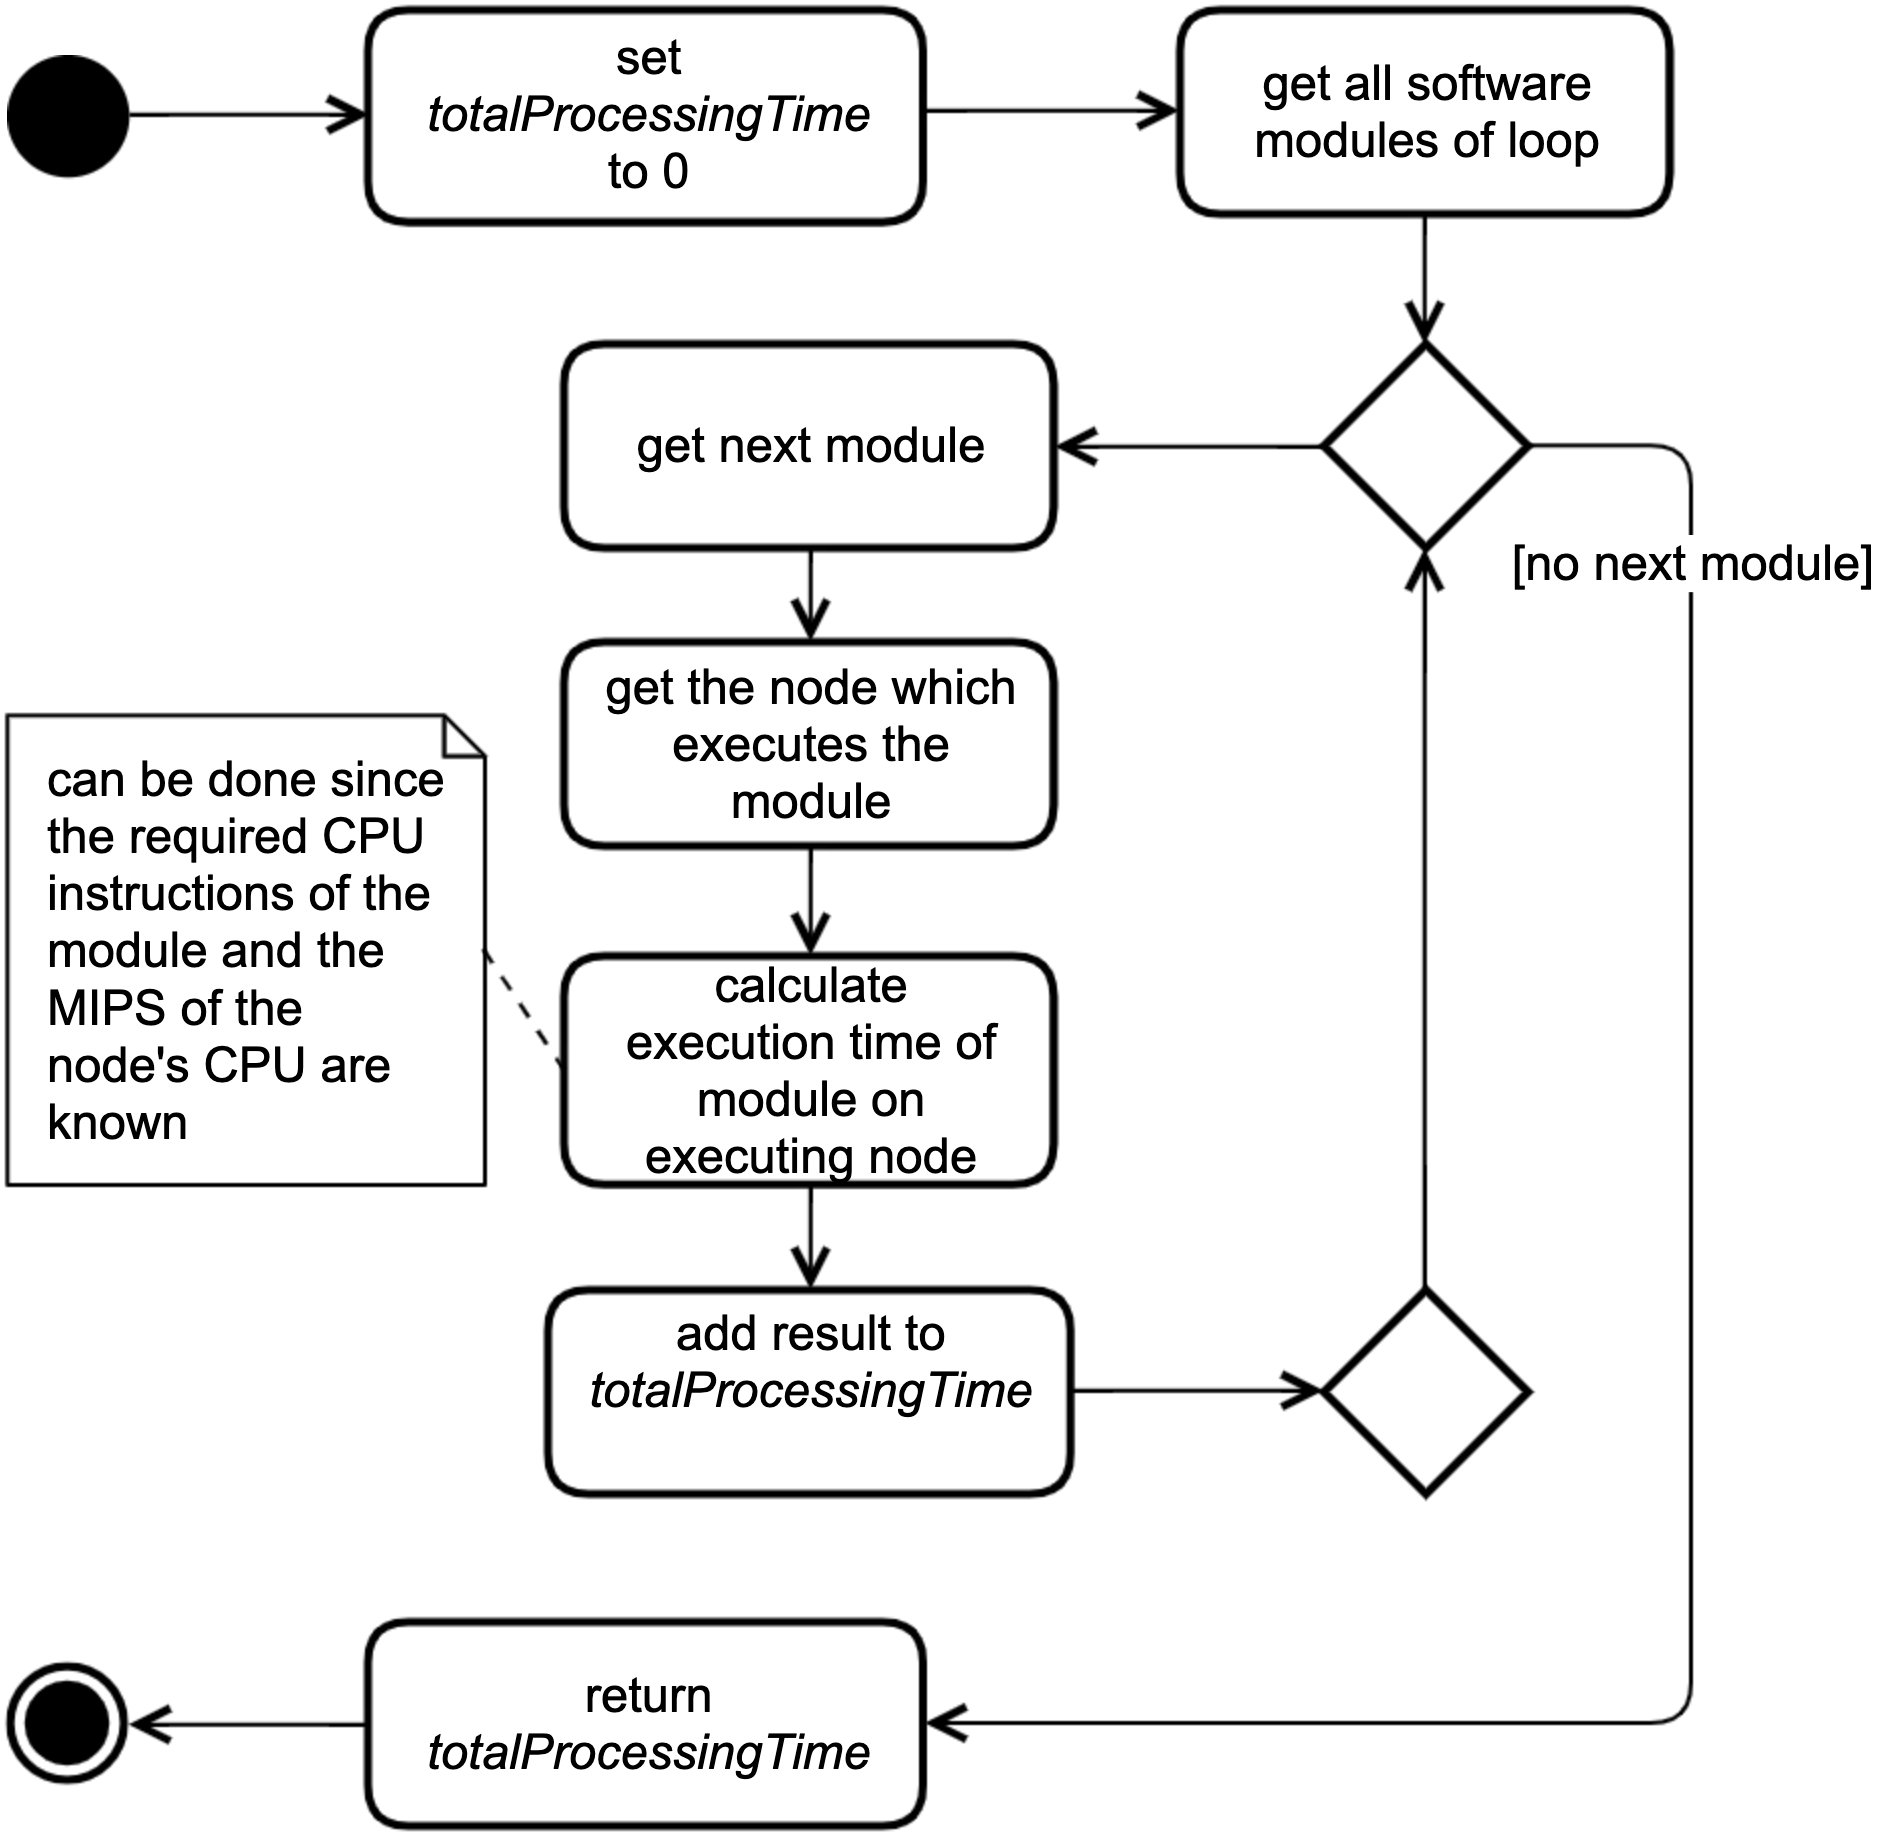
\includegraphics[width=0.9\textwidth]{algorithm-activitydiagram-latency-processing}
    \caption{Activity diagram for calculating the total processing time of a loop}
    \label{fig:algorithm-activitydiagram-latency-processing}
\end{figure}

\begin{figure}[htb]
    \centering
    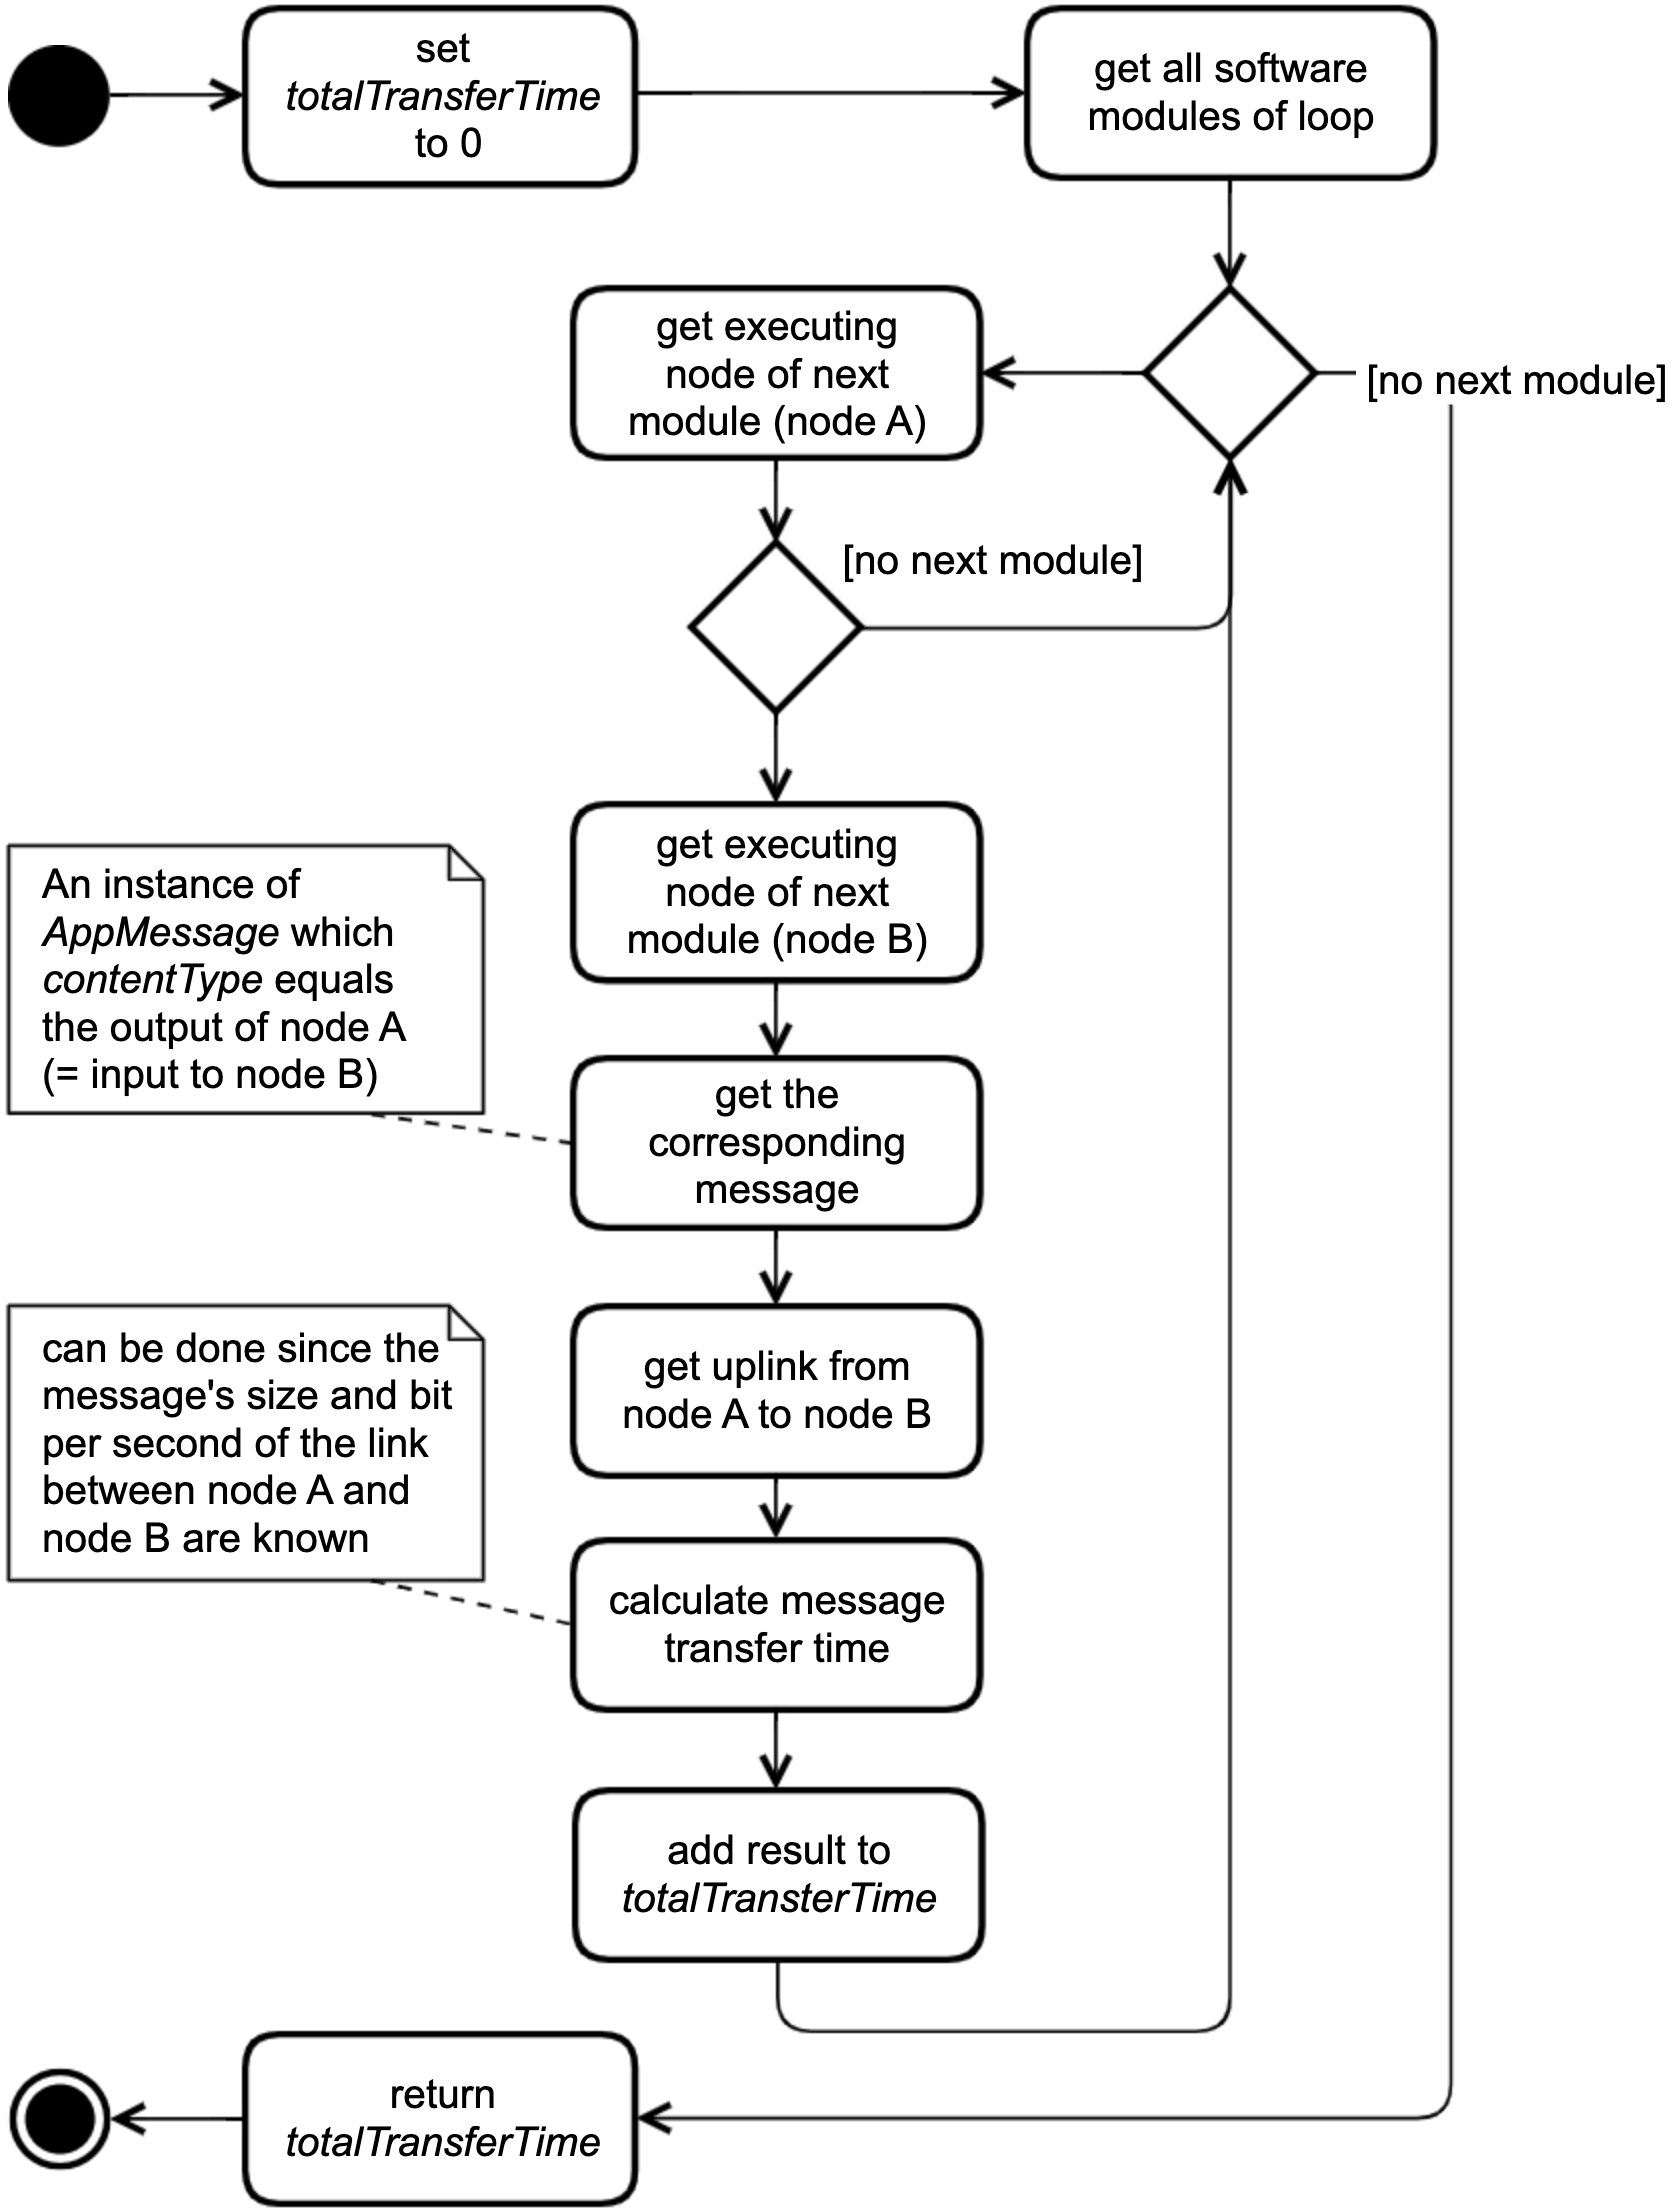
\includegraphics[width=0.9\textwidth]{algorithm-activitydiagram-latency-transfer}
    \caption{Activity diagram for calculating the total transfer time of messages between nodes of a loop}
    \label{fig:algorithm-activitydiagram-latency-transfer}
\end{figure}

\begin{figure}[htb]
    \centering
    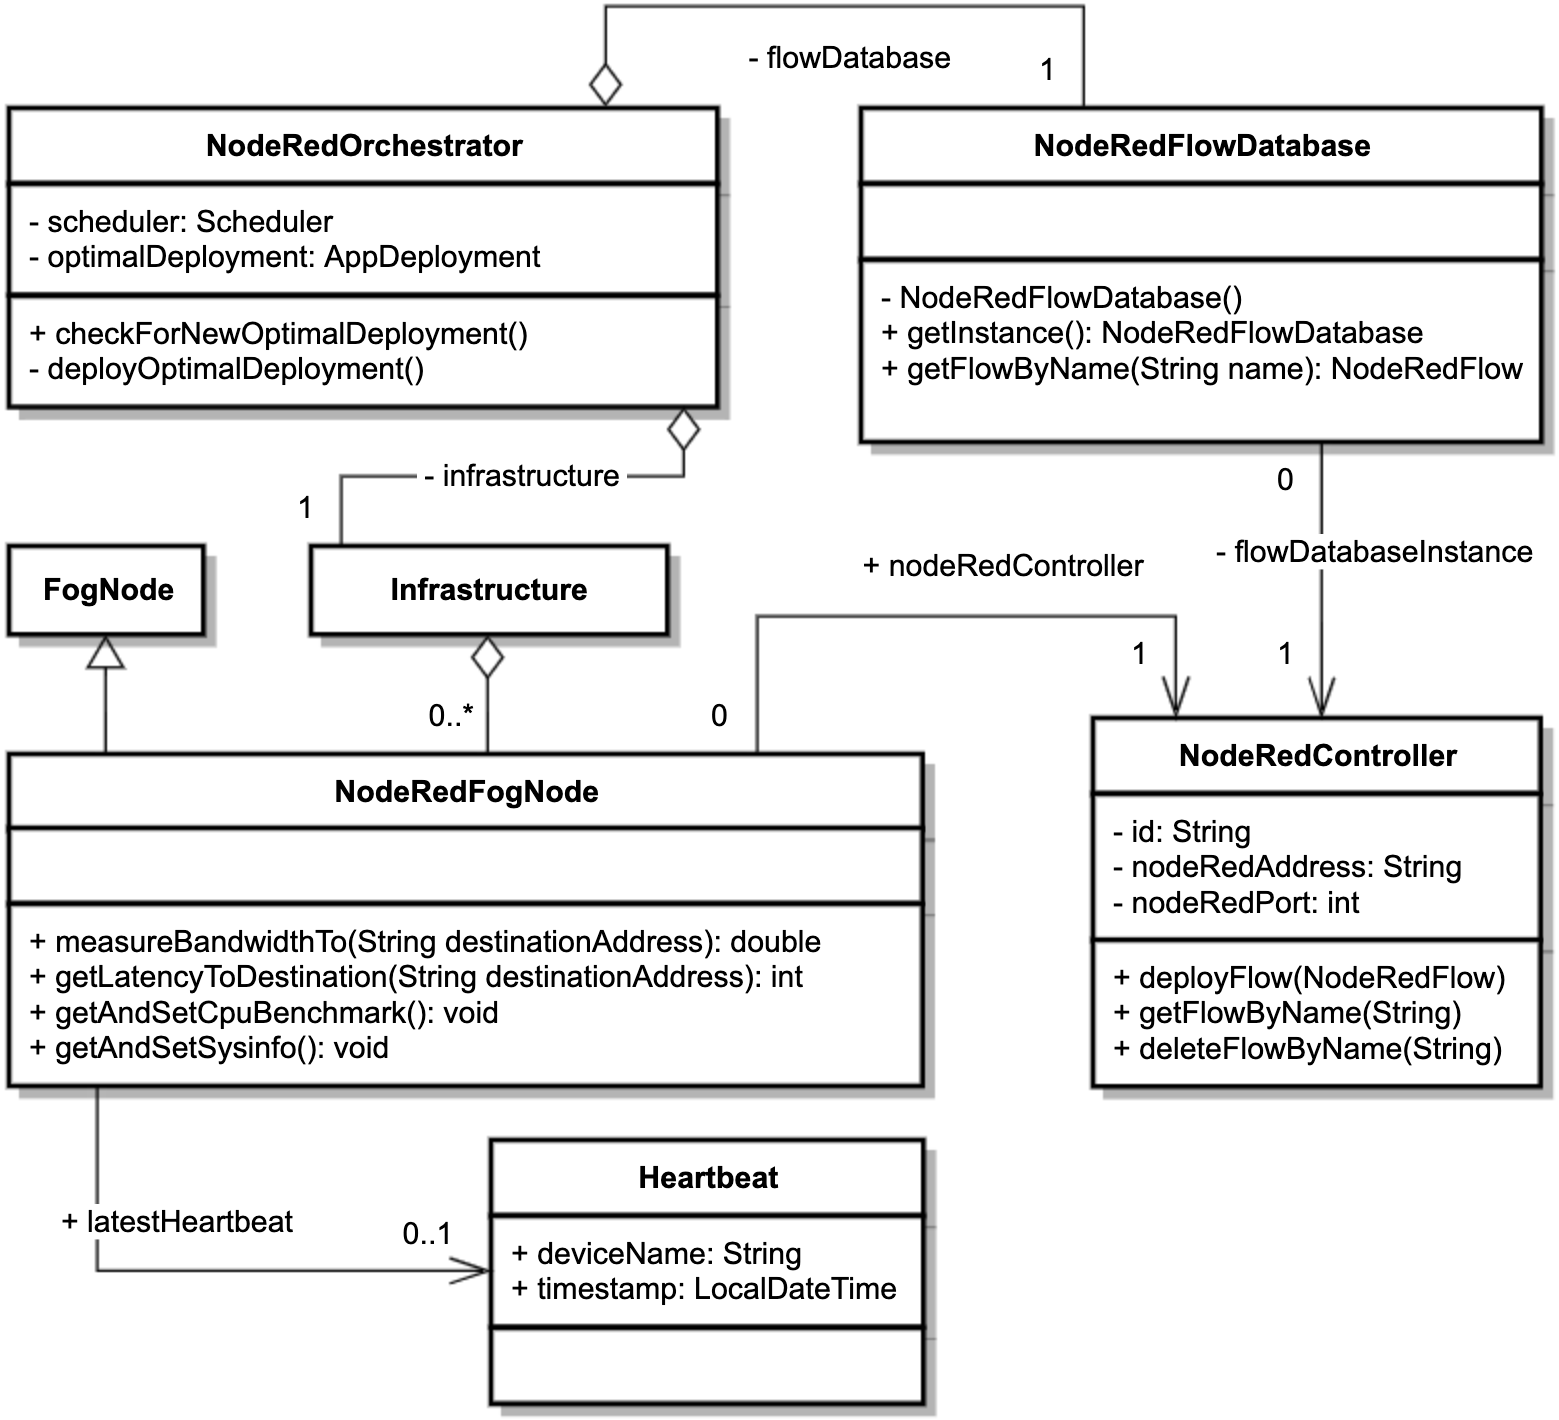
\includegraphics[width=1.0\textwidth]{orchestrator-classdisgram}
    \caption{Class diagram of \texttt{NodeRedOrchestrator}}
    \label{fig:orchestrator-classdisgram}
\end{figure}
    
    \backmatter




\end{document}